\documentclass[11pt, a4]{article}
\newcommand{\lotteryset}{\mathcal{L}}
\newcommand{\outcomeset}{\mathcal{X}}
\usepackage{amssymb}
\usepackage{enumitem}
\usepackage{amsmath}
\usepackage{tfrupee}
\usepackage{pgfplots}
\usepackage{tikz}
\usepackage{enumitem}
\usepackage{multirow}
\usepackage{fancyhdr}
\usepackage{lastpage}
\usepackage[export]{adjustbox}
\usepackage{wrapfig}
\usepackage[english]{babel}
\usepackage{amsthm}
\usepackage{multirow}
\usepackage{wrapfig,lipsum,booktabs}
\usepackage{graphicx}
\usepackage{subcaption} 
\usepackage{float}
\usepackage{hyperref}

\topmargin -0.4in
% \textheight 11in
\oddsidemargin .0in
\evensidemargin 0.0in
\textwidth 6.5in

\begin{document}
	\pagestyle{fancy}
	\fancyhead{}\fancyfoot{}
	\fancyhead[L]{PA-1 Report}
	\fancyhead[C]{\thepage ~of \pageref{LastPage}}
	\fancyhead[R]{EE25S009}
	\author{Ritabrata Mandal\\ EE25S009}
	\title{EE5176: Computational Photography\\Programming Assignment-1: Basics of Imaging Report}
	\maketitle
	
	\medskip
	\newpage
	\begin{enumerate}
		\item \textbf{Introduction}\\
		This assignment focuses on fundamental concepts in digital imaging, beginning with demosaicing and extending to noise removal. 
		All processed images generated during the assignment are available in the GitHub repository under the 
		\href{URL}{\texttt{output}} folder.  
		
		\begin{enumerate}
			\item \textbf{Implementation}:\\
			The implementation has been carried out and tested in MATLAB R2025a. 
			A \texttt{main.m} script invokes four functions: \texttt{demos.m}, \texttt{white\_balance.m}, 
			\texttt{tone\_map.m}, and \texttt{denoising.m}. 
			The \texttt{demos.m} function performs image demosaicing for two given raw images, \texttt{RawImage1} and \texttt{RawImage2}. 
			The functions \texttt{white\_balance.m} and \texttt{tone\_map.m} apply white balancing and tone mapping techniques, respectively, 
			on images such as \texttt{RawImage1} and \texttt{kodim19}. 
			
			\item \textbf{Running the Code}:\\
			To execute the assignment, navigate to the \texttt{Assignment1} directory, run the \texttt{main.m} file, 
			and select options \texttt{1}, \texttt{2}, or \texttt{3} corresponding to the three tasks.
		\end{enumerate}
		
		\item \textbf{Demosaicing}\\
		Demosaicing is a process of interpolating the red, green and blue channels from
		the raw pixel image. Here we will try to ll in the missing pixel values from
		the sampled raw images through interpolation. \\
		 The CFA for \texttt{RawImage1.mat} is rggb whose mask is provided in the le
		\texttt{bayer1.mat}. In\texttt{ bayer1.mat} a value of 1 at a particular pixel means that only
		red value is sampled at that pixel. Similarly values of 2 and 3 mean that
		only green and blue values are sampled at those pixels. We use bilinear and
		bicubic interpolation for filling in the missing data. We interpolate only for
		those pixels whose values are missing in the grid. We use the MATLAB built-in
		function \texttt{griddata} for an efficient implementation.
		\begin{enumerate}
			\item Performing bilinear interpolation of the missing pixels in each color channel	R, G and B to reconstruct a full color image from RawImage1 with the CFA provided in \texttt{bayer1.mat} and figure-\ref{fig:problem1_linear} shows the different color channel after interpolation. Figure~\ref{fig:problem1_RGB_linear} shows the RGB reconstruction with linear interpolation
			\begin{figure}[h]
				\centering
				\resizebox{0.8\linewidth}{!}{
					\begin{tabular}{cc}
					\begin{subfigure}[h]{0.45\linewidth}
						\centering
						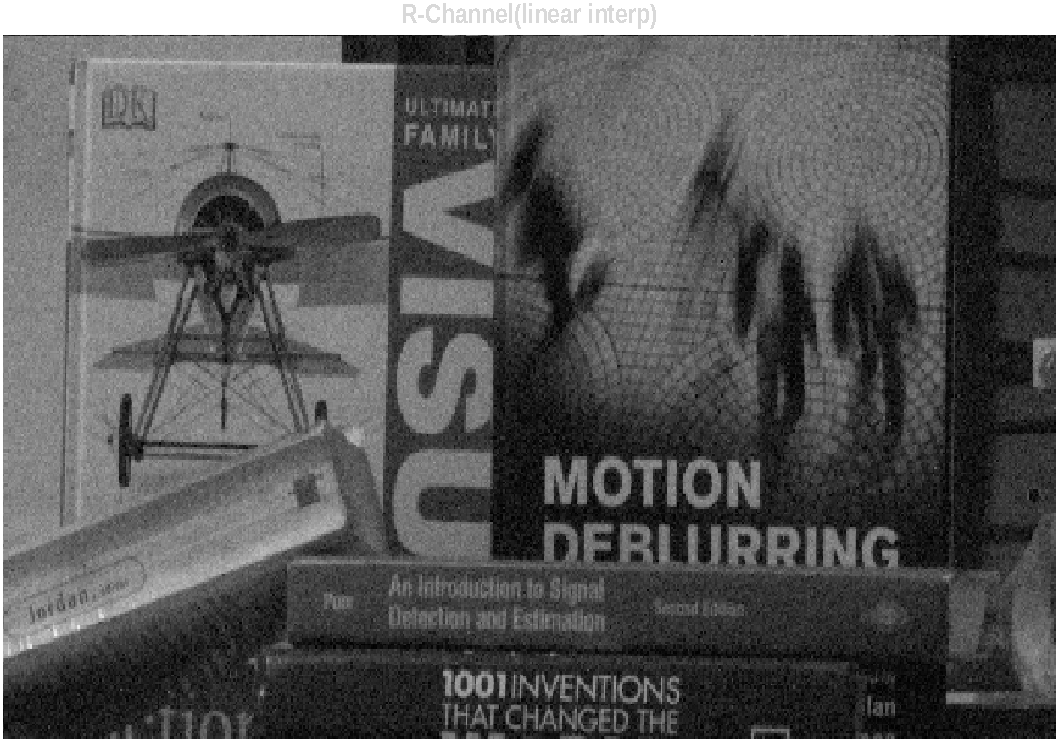
\includegraphics[width=\linewidth]{../output/1_R-channel_linear.pdf}
						\caption{R-Channel}
						\label{fig:problem1_R}
					\end{subfigure} &
					\begin{subfigure}[h]{0.45\linewidth}
						\centering
						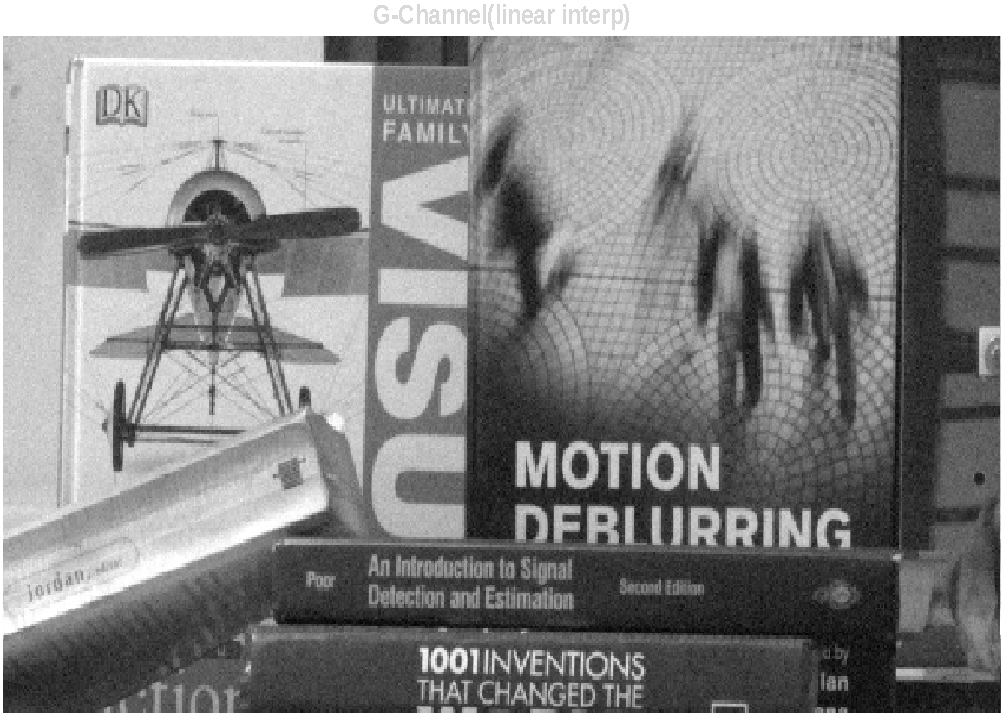
\includegraphics[width=\linewidth]{../output/1_G-channel_linear.pdf}
						\caption{G-Channel}
						\label{fig:problem1_G_linear}
					\end{subfigure}\\
					\begin{subfigure}[h]{0.45\linewidth}
						\centering
						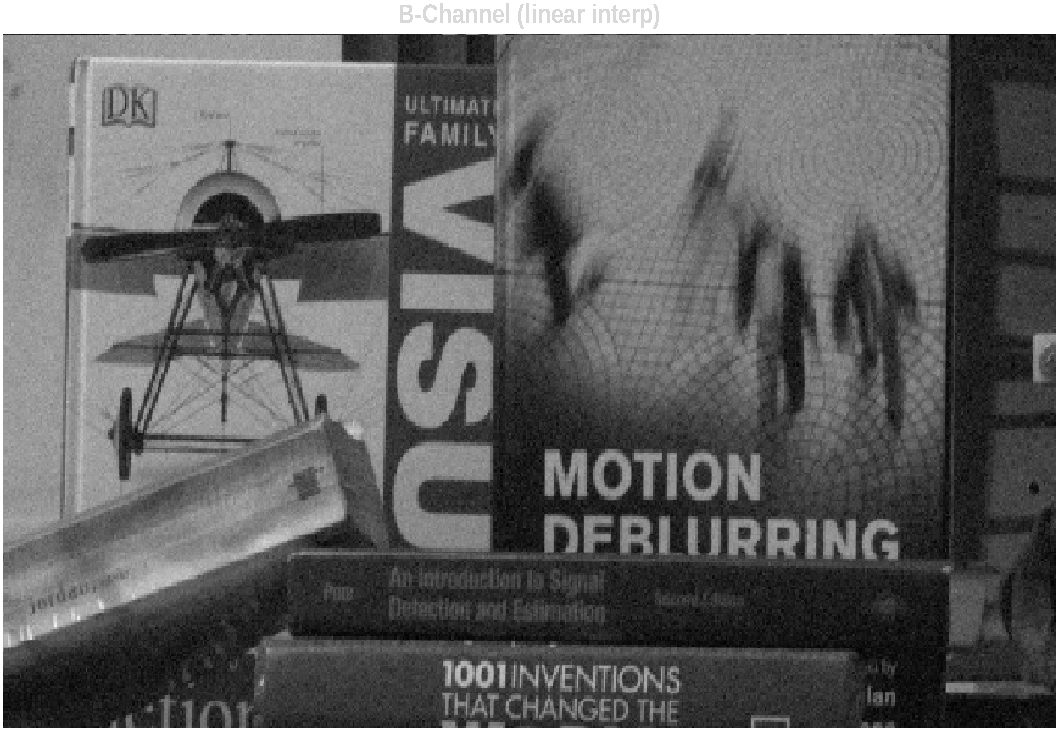
\includegraphics[width=\linewidth]{../output/1_B-channel_linear.pdf}
						\caption{B-Channel}
						\label{fig:problem1_B_linear}
					\end{subfigure} &
					\begin{subfigure}[h]{0.45\linewidth}
						\centering
						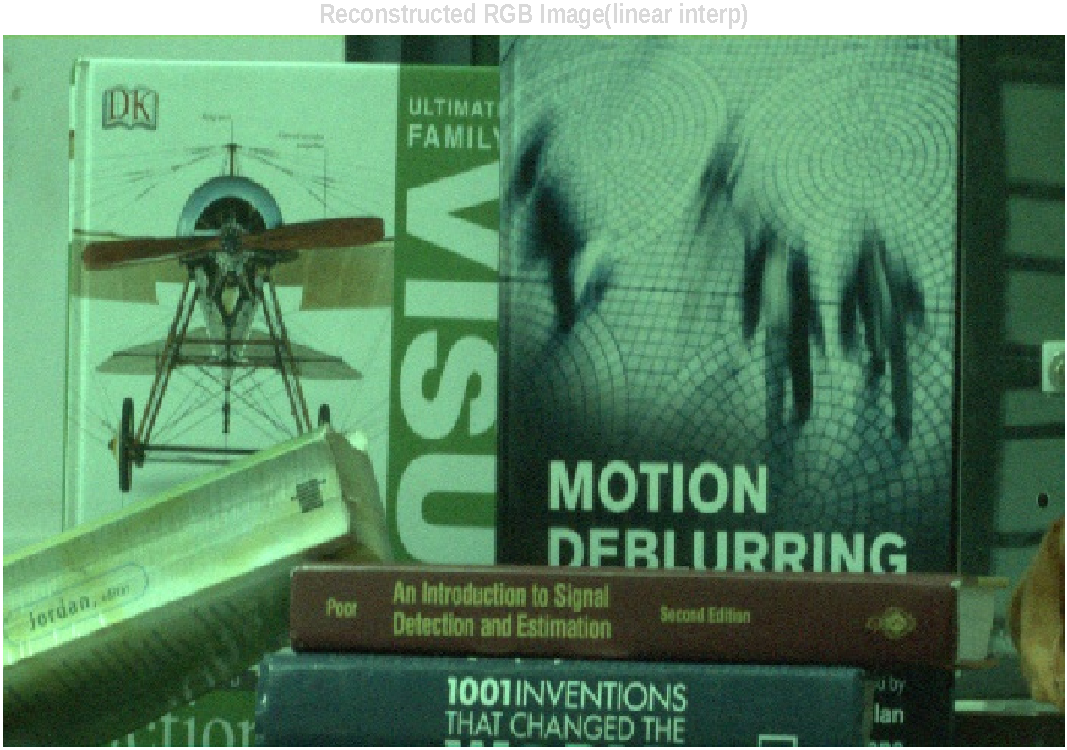
\includegraphics[width=\linewidth]{../output/1_RGB_linear.pdf}
						\caption{Reconstructed	RGB}
						\label{fig:problem1_RGB_linear}
					\end{subfigure}
				\end{tabular}
			}
%				\label{fig:problem1_linear}
				\caption{Reconstructed \texttt{RawImage1} with linear interpolation.}
				\label{fig:problem1_linear}
			\end{figure}
			
			\item  Performing bicubic interpolation of the missing pixels in each color channel	R, G and B to reconstruct a full color image from RawImage1 with the CFA provided in \texttt{bayer1.mat} and figure-\ref{fig:problem1_cubic} shows the different color channel after interpolation. Figure~\ref{fig:problem1_RGB_cubic} shows the RGB reconstruction with cubic interpolation.\\
			\textbf{Comparision with Bilinear Interpolation:} When comparing the results of bicubic interpolation and bilinear interpolation, the images appear almost identical at first glance. However, on closer inspection by zooming in, bicubic interpolation produces sharper edges with less blurriness than bilinear interpolation. In general, unless we specifically look for these differences at higher magnification, it is difficult to distinguish between the two images.
			
			\begin{figure}[H]
				\centering
				\resizebox{0.8\linewidth}{!}{ 
					\begin{tabular}{cc}
						\begin{subfigure}[h]{0.45\linewidth}
							\centering
							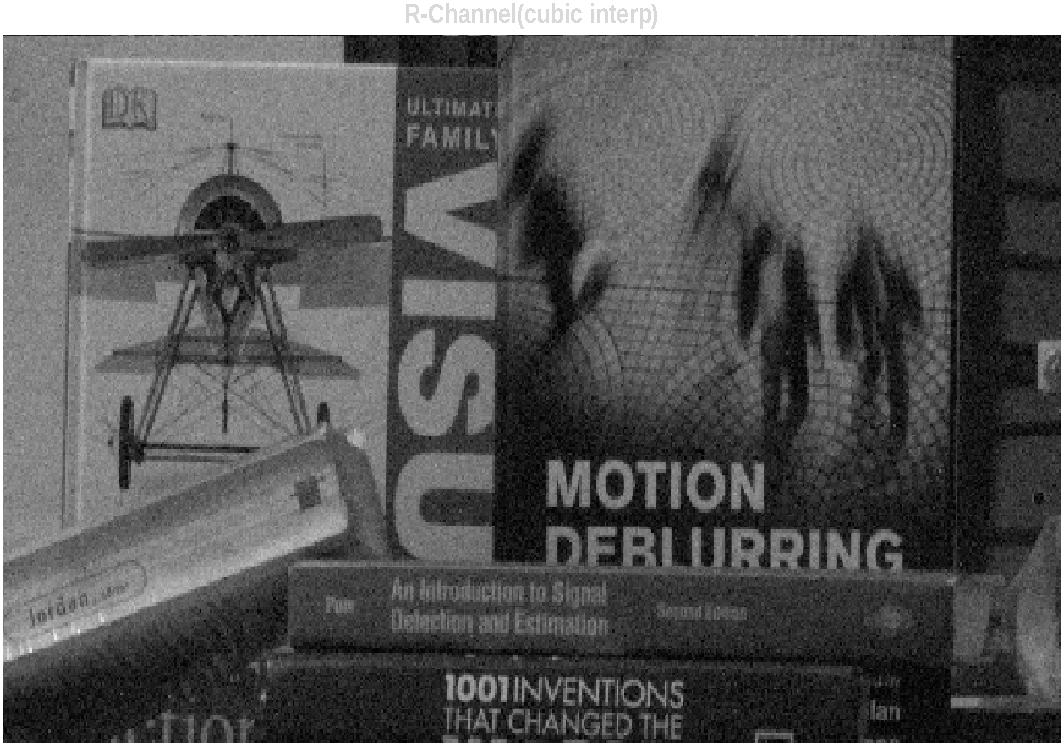
\includegraphics[width=\linewidth]{../output/1_R-channel_cubic.pdf}
							\caption{R-Channel}
							\label{fig:problem1_R_cubic}
						\end{subfigure} &
						\begin{subfigure}[h]{0.45\linewidth}
							\centering
							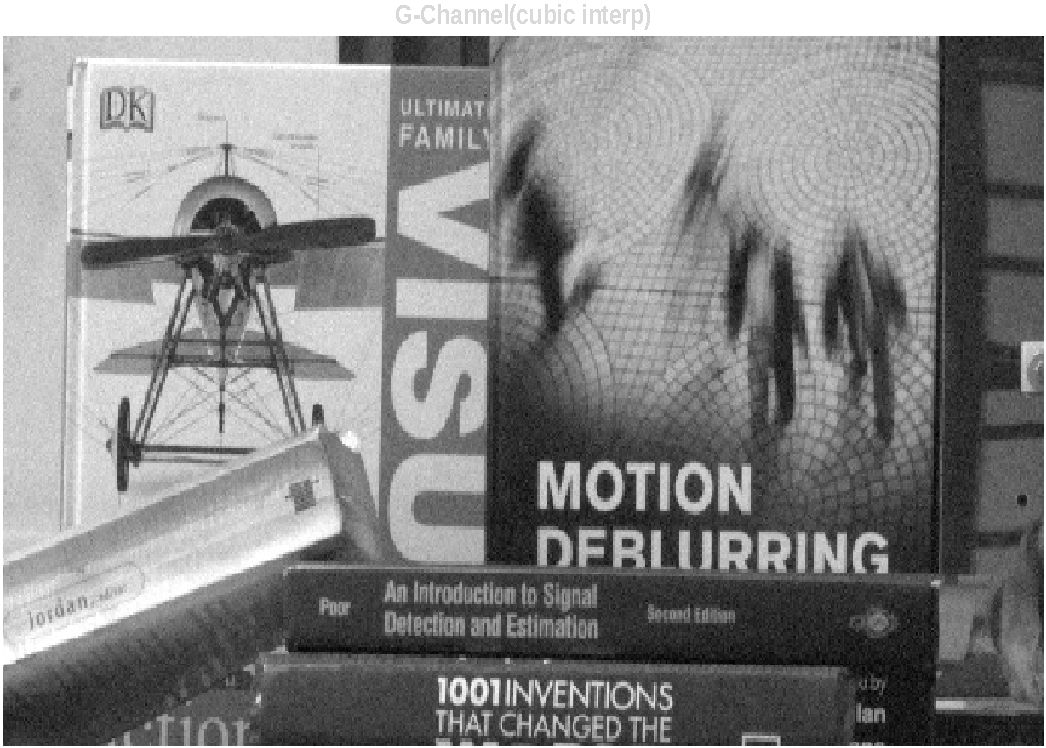
\includegraphics[width=\linewidth]{../output/1_G-channel_cubic.pdf}
							\caption{G-Channel}
							\label{fig:problem1_G_cubic}
						\end{subfigure} \\
						\begin{subfigure}[h]{0.45\linewidth}
							\centering
							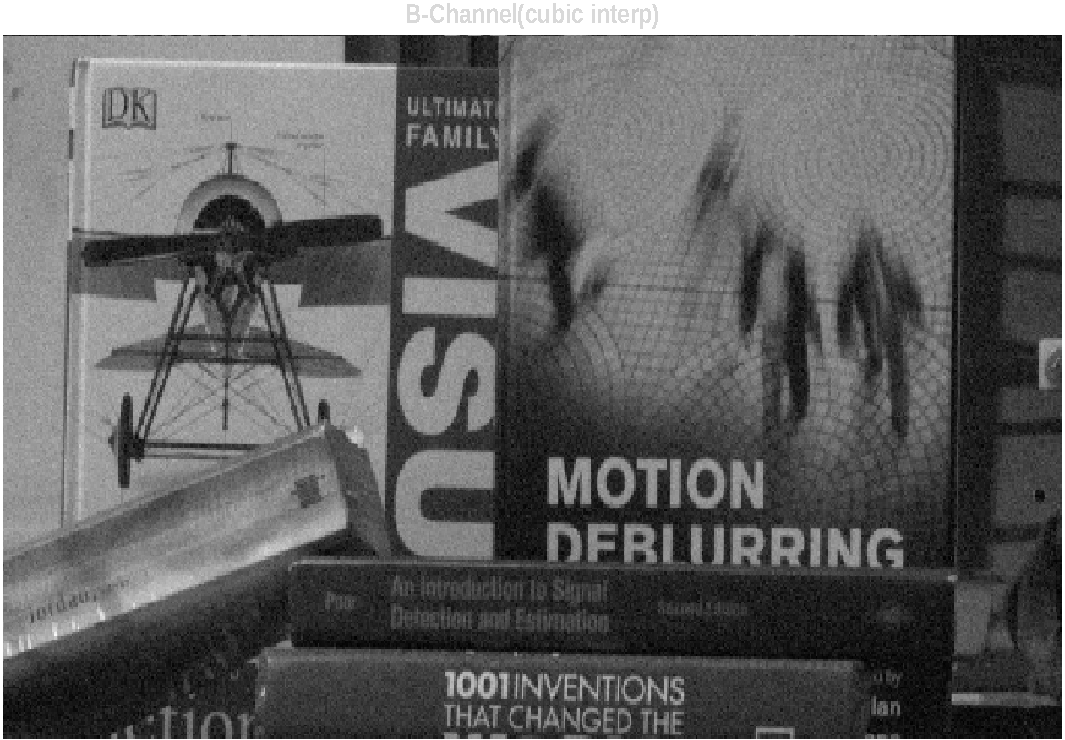
\includegraphics[width=\linewidth]{../output/1_B-channel_cubic.pdf}
							\caption{B-Channel}
							\label{fig:problem1_B_cubic}
						\end{subfigure} &
						\begin{subfigure}[h]{0.45\linewidth}
							\centering
							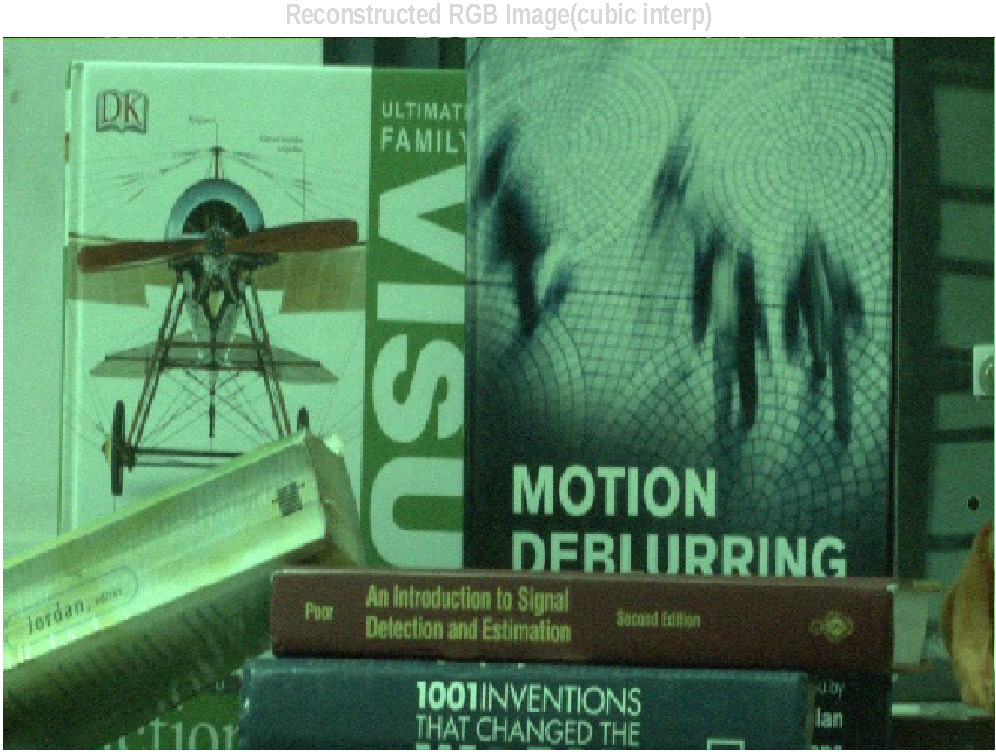
\includegraphics[width=\linewidth]{../output/1_RGB_cubic.pdf}
							\caption{Reconstructed RGB}
							\label{fig:problem1_RGB_cubic}
						\end{subfigure}
					\end{tabular}
				}
				\caption{Reconstructed \texttt{RawImage1} with cubic interpolation.}
				\label{fig:problem1_cubic}
			\end{figure}
			
			\item As shown in Figure~\ref{fig:problem1_inbuild}, the \texttt{RawImage1} was demosaiced using the rggb pattern with MATLAB’s built-in function \texttt{demosaic}.\\
			\textbf{Comparison with Interpolation Methods:}\\
			The three interpolation methods produce images that look quite similar, with differences only noticeable upon zooming in. In such cases, the \texttt{demosaic} function retains edge information more effectively, giving sharper results. Since \texttt{RawImage1} contains little high-frequency content, even bilinear interpolation performs well, though tone-mapped outputs from \texttt{demosaic} show a purple hue compared to the more neutral colors of bicubic interpolation.  
			
			
			\begin{figure}[H]
				\centering
				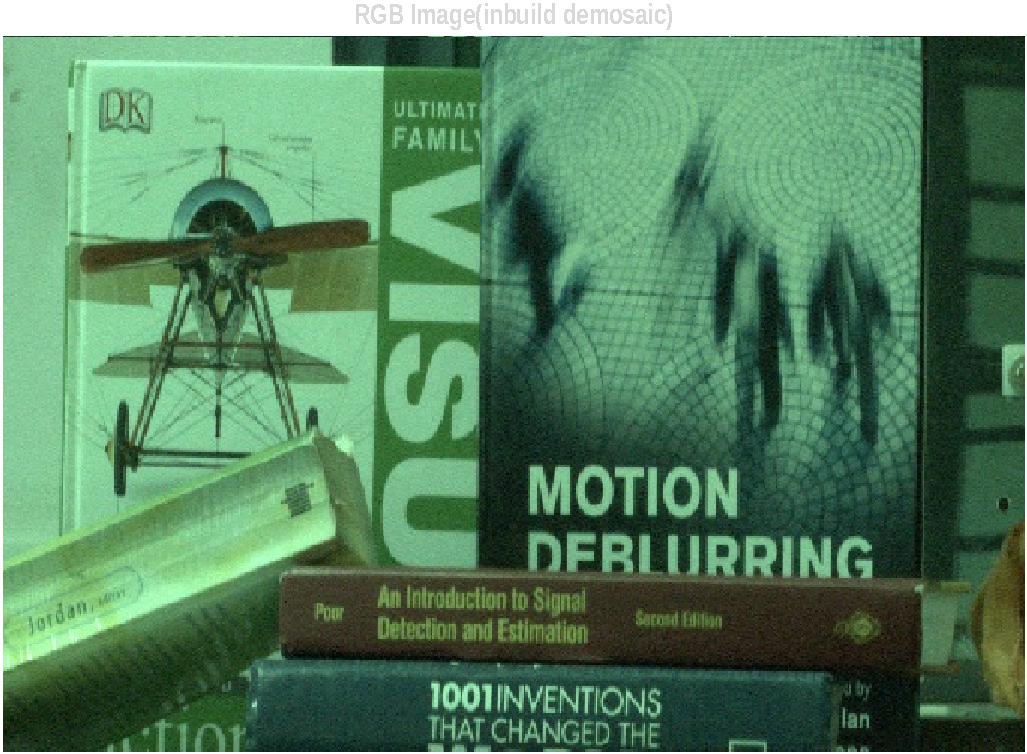
\includegraphics[width=0.5\linewidth]{../output/1_RGB_inbuild.pdf}
				\caption{Reconstructed \texttt{RawImage1} with \texttt{demosaic} function}
				\label{fig:problem1_inbuild}
			\end{figure}
			\item \textbf{Assumptions in Interpolation of Missing Pixel Values:}  
			\begin{enumerate}
				\item \textbf{Local Smoothness:} The image intensity is assumed to vary smoothly in a local neighborhood.  
				\item \textbf{Correlation of Neighboring Pixels:} Adjacent pixels are assumed to have similar values, especially within homogeneous regions.  
				\item \textbf{Limited High-Frequency Content:} The image is assumed to have relatively low noise and not contain abrupt intensity changes at small scales.  
				\item \textbf{Edge Continuity:} Edges are assumed to be continuous, allowing interpolation methods to preserve structure without introducing artifacts.  
			\end{enumerate}
			
			\textbf{Consequences When Assumptions Do Not Hold:}  
			\begin{enumerate}
				\item \textbf{Loss of Detail:} If the image has high-frequency textures, interpolation may blur fine details.  
				\item \textbf{Artifacts:} Discontinuities in intensity (e.g., at edges) may cause artifacts such as color fringing or checkerboard patterns.  
				\item \textbf{Distortion of Structures:} Interpolated pixels may not follow the true underlying structure, leading to edge distortion.  
				\item \textbf{Noise Amplification:} In the presence of noise, interpolation may reinforce or spread the noise instead of reconstructing the true signal.  
			\end{enumerate}
			
			\item Performing bicubic interpolation on \texttt{kodim19.mat} which has been sampled
			with the CFA pattern ‘RGGB’ to reconstruct a full color image shown in Figure~\ref{fig:problem1_part2}.
			\begin{figure}[h]
				\centering
				\resizebox{0.8\linewidth}{!}{
					\begin{tabular}{cc}
					\begin{subfigure}[h]{0.45\linewidth}
						\centering
						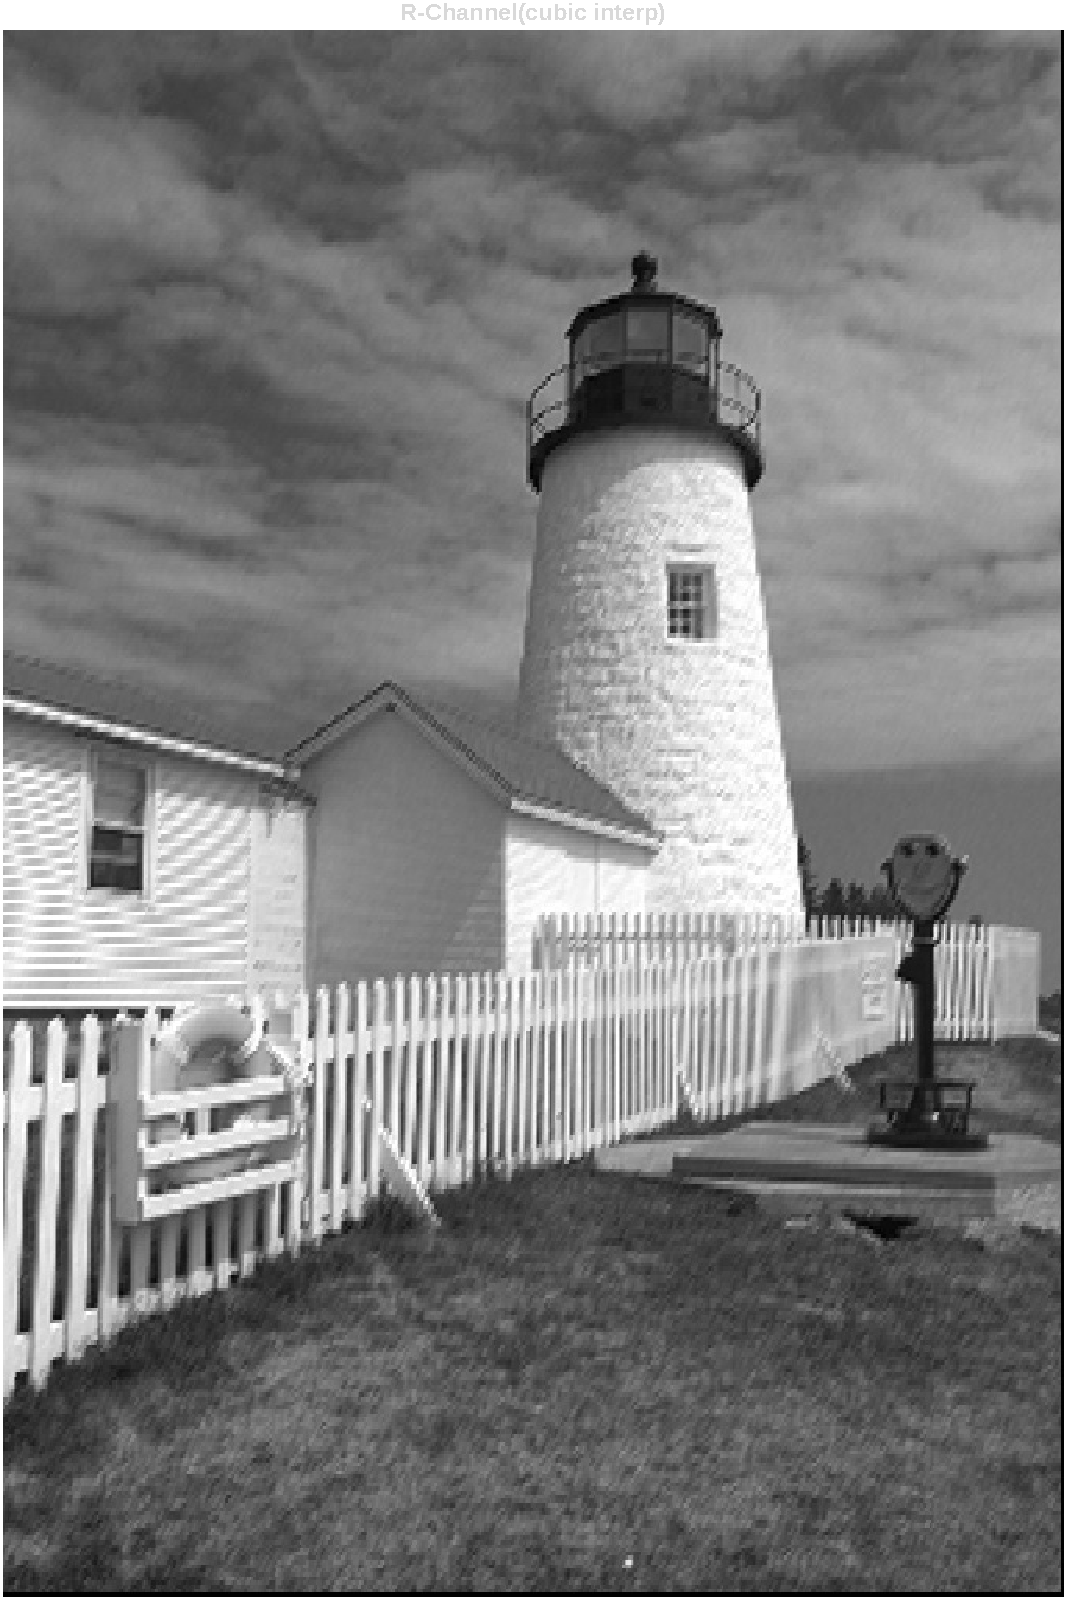
\includegraphics[width=\linewidth]{../output/2_R-channel_cubic.pdf}
						\caption{R-Channel}
						\label{fig:problem1_part2_R_cubic}
					\end{subfigure} &
					\begin{subfigure}[h]{0.45\linewidth}
						\centering
						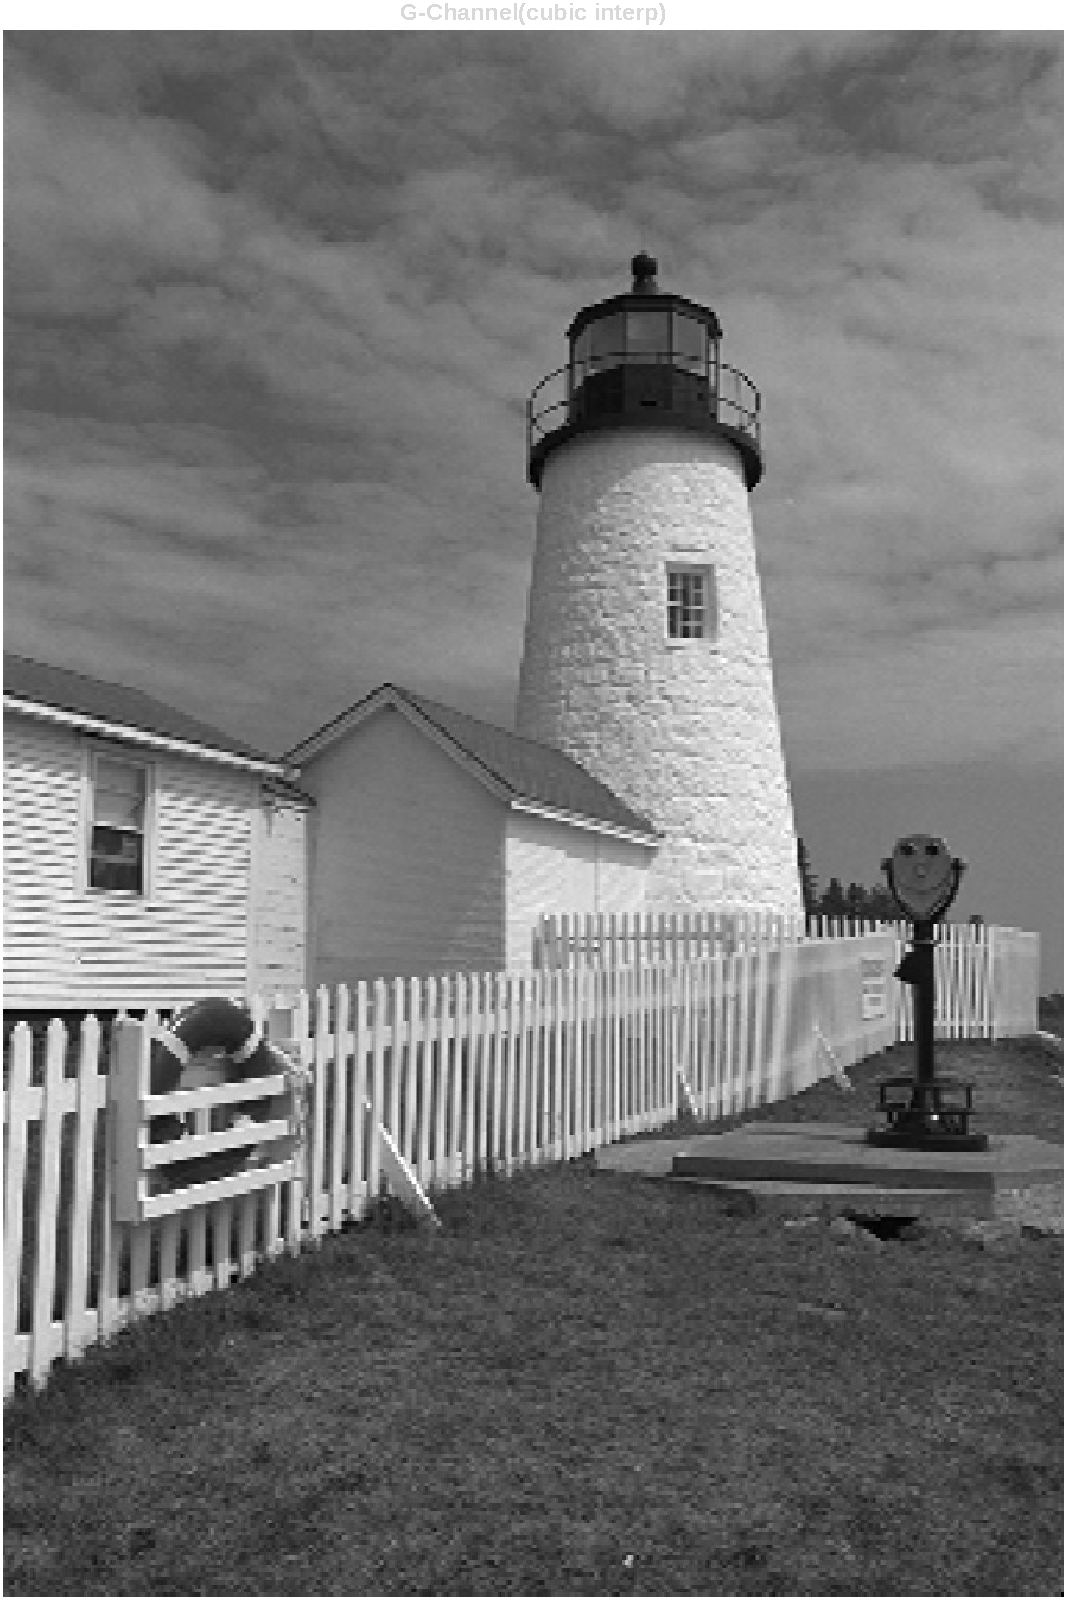
\includegraphics[width=\linewidth]{../output/2_G-channel_cubic.pdf}
						\caption{G-Channel}
						\label{fig:problem_part21_G_cubic}
					\end{subfigure}\\
					\begin{subfigure}[h]{0.45\linewidth}
						\centering
						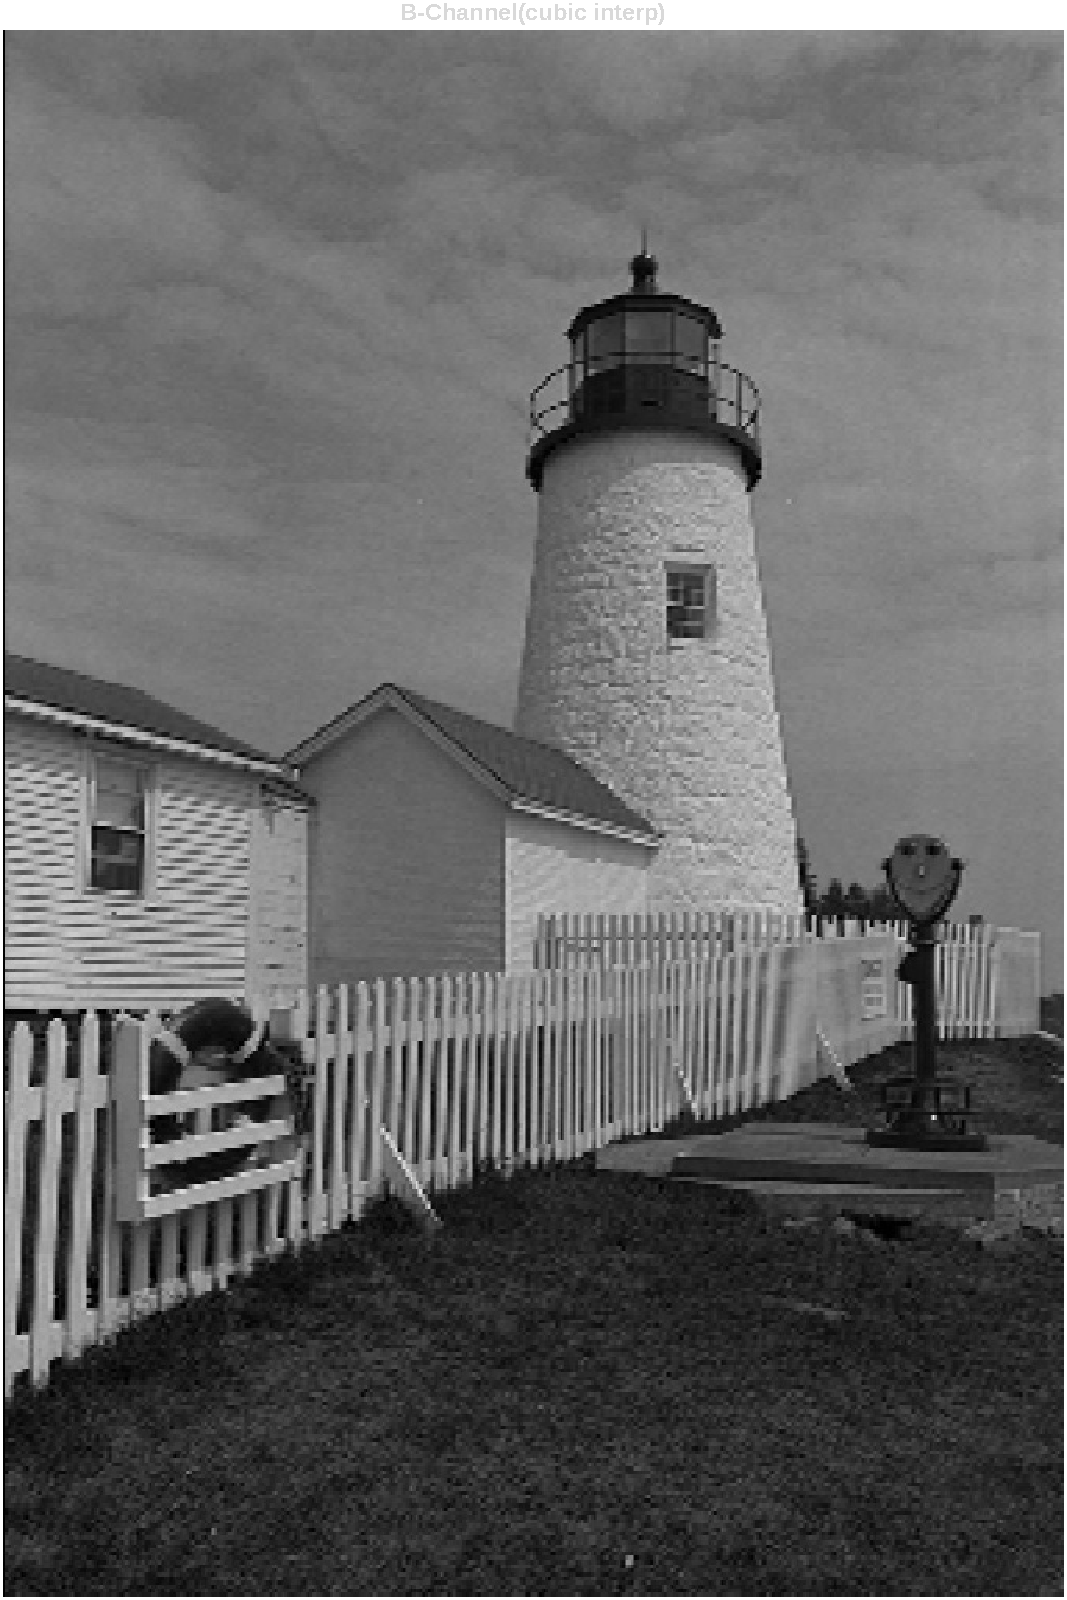
\includegraphics[width=\linewidth]{../output/2_B-channel_cubic.pdf}
						\caption{B-Channel}
						\label{fig:problem1_part2_B_cubic}
					\end{subfigure} &
					\begin{subfigure}[h]{0.45\linewidth}
						\centering
						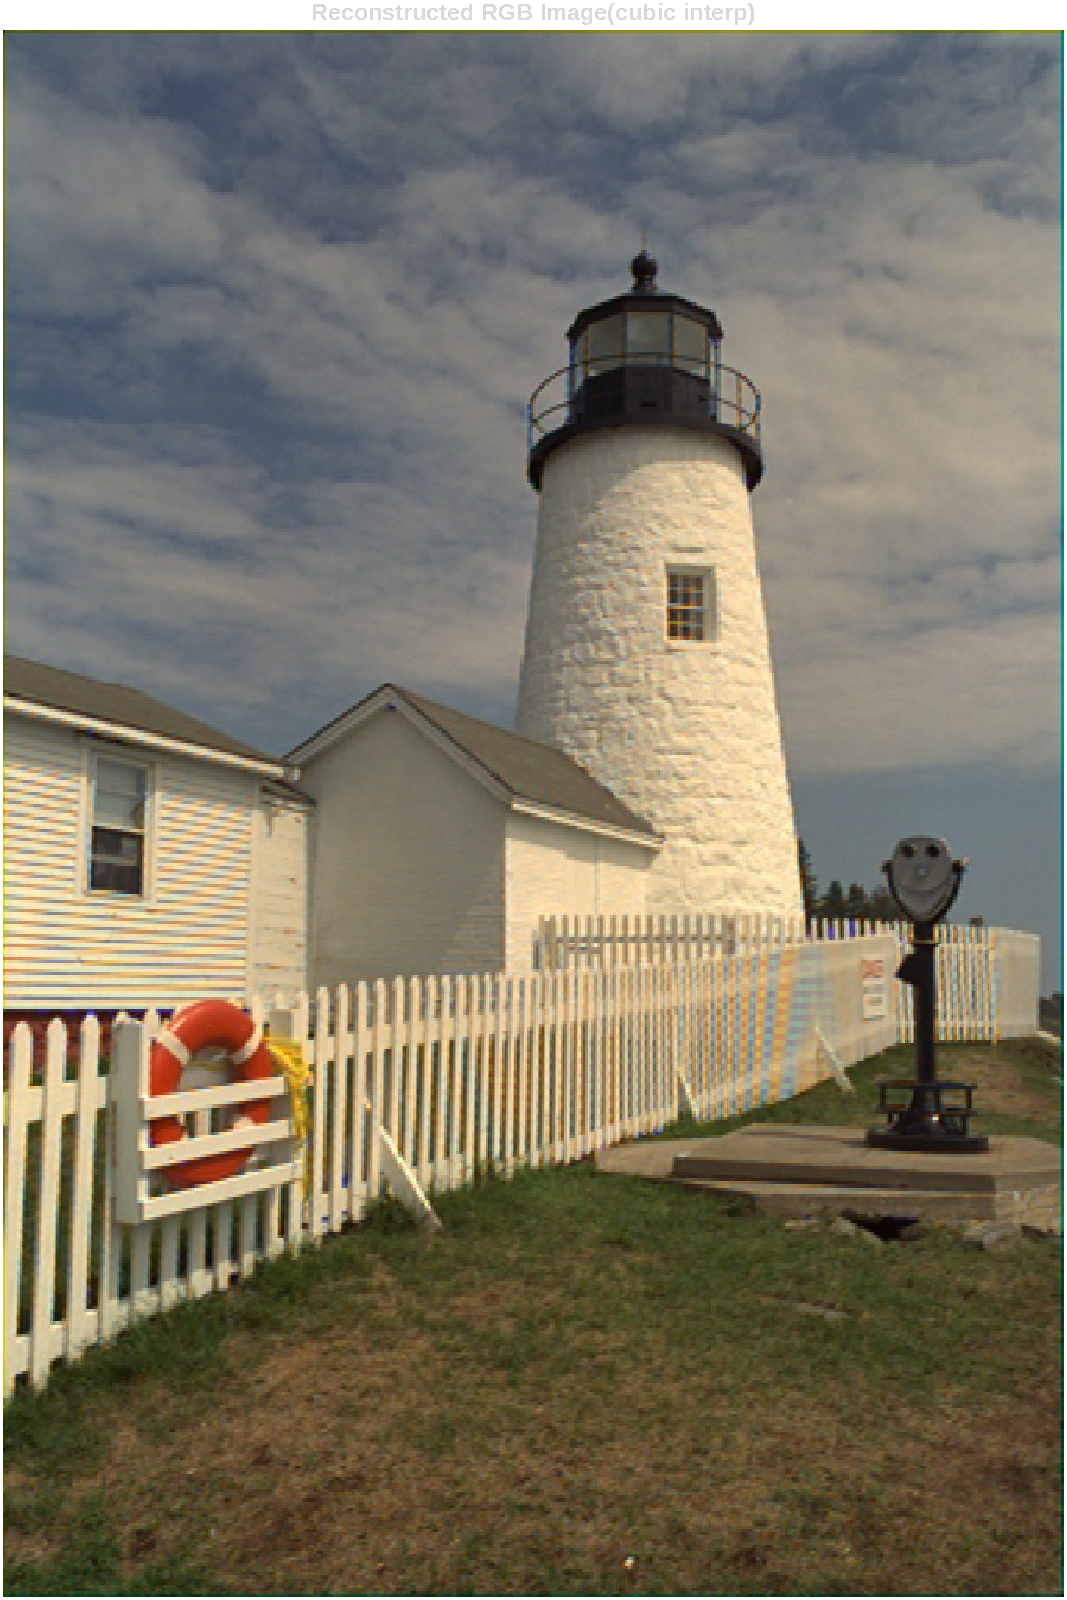
\includegraphics[width=\linewidth]{../output/2_RGB_cubic.pdf}
						\caption{Reconstructed RGB}
						\label{fig:problem1_part2_cubic}
					\end{subfigure}
					\end{tabular}
				}
				\caption{Reconstructed \texttt{kodim19.mat} with cubic interpolation.}
				\label{fig:problem1_part2}
			\end{figure}
			\item Now taking the Figure \ref{fig:problem1_part2_cubic} converting to YCrCb and applying the median filter to the chrominance channels and then converting back it to RGB channel I get Figure~\ref{fig:problem1_part2_with_median}
			\begin{figure}[h]
				\centering
				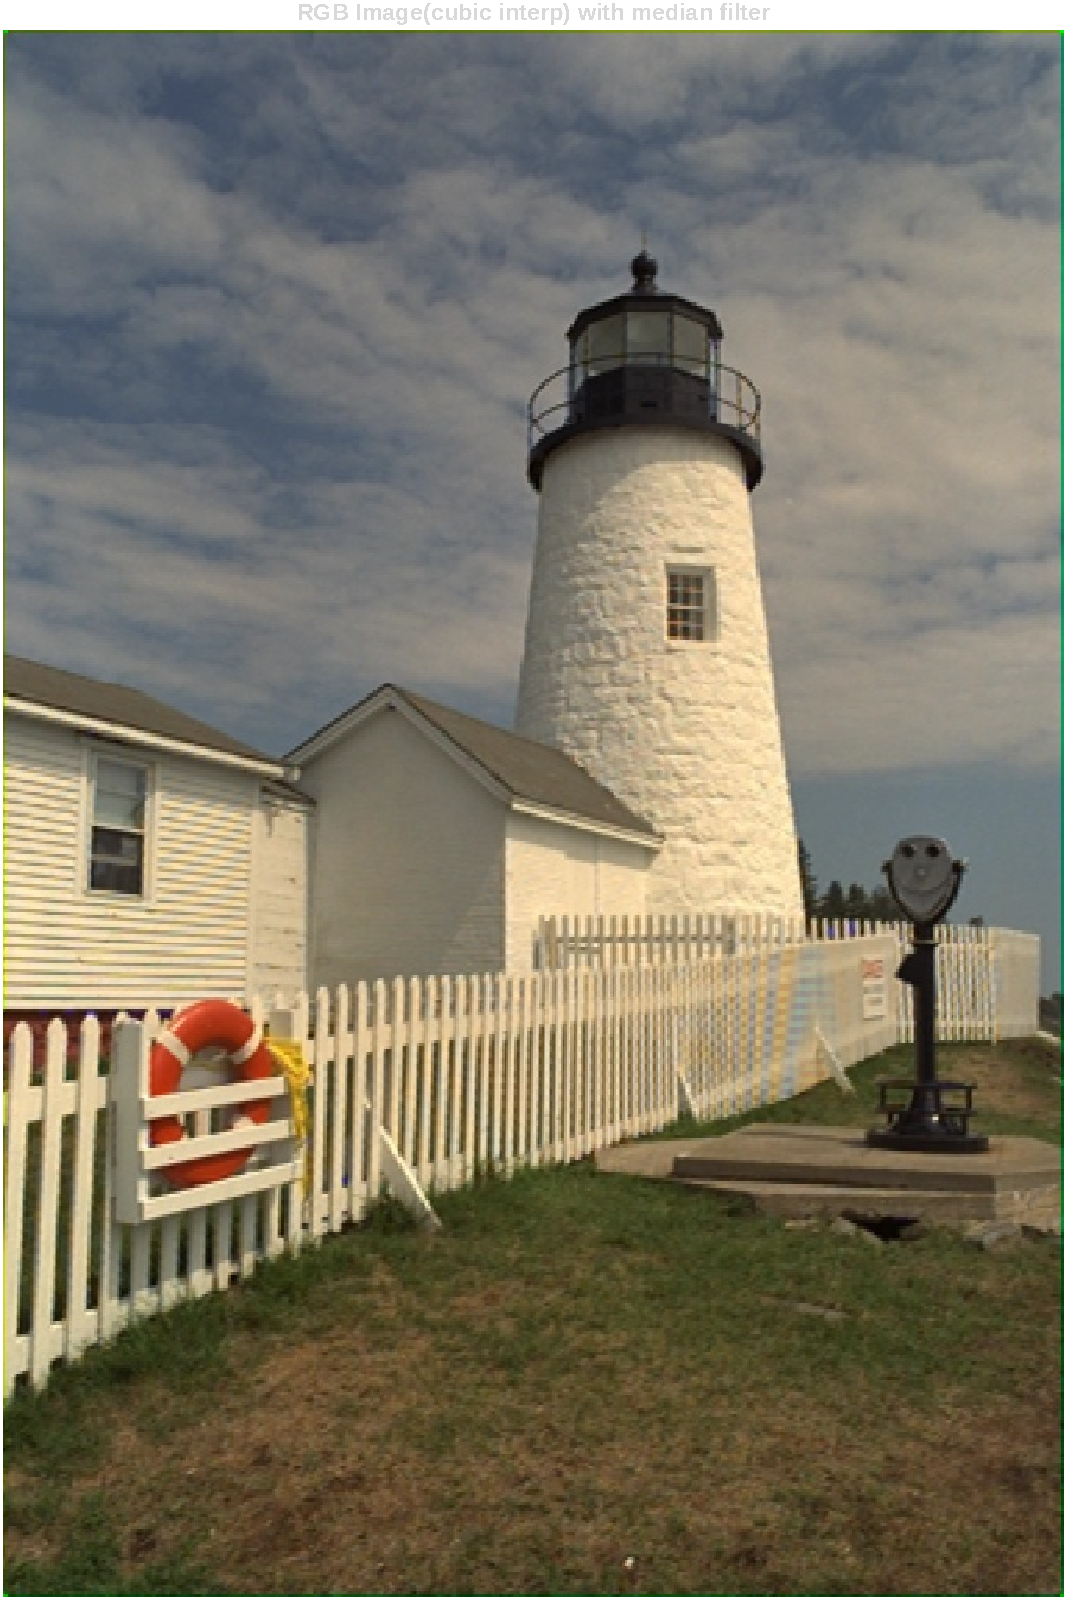
\includegraphics[width=0.5\linewidth]{../output/2_RGB_cubic_median.pdf}
				\caption{After applying the Median filter to the chrominance channel.}
				\label{fig:problem1_part2_with_median}
			\end{figure}
			\item in the \ref{fig:problem1_part2_cubic} image (i.e. cubic interpolated rgb) we can see the moire pattern where as in \ref{fig:problem1_part2_with_median} image (i.e. after applying median filter in chrominance channel) there is no moire pattern in the image.
		\end{enumerate}
		\item \textbf{White Balancing and Tone Mapping}\\
		In this section we do white balance and tone mapping for images \texttt{RawImage1}, \texttt{RawImage2} and \texttt{RawImage3}. In build \texttt{demosaic} function is used to demosaic the images. There are basically three ways to do white balancing.
		\begin{itemize}
			\item Assume the average color of the scene to be gray and then do white balancing. 
			\item Assume that the brightest pixel is a specular highlight and hence should
			therefore be white
			\item Assume that some part of the scene to be neutral.
		\end{itemize}
		 After white balancing the images, tone mapping is performed on them. We try
		two methods of tone mapping.
		\begin{itemize}
			\item Histogram equalization
			\item Gamma correction for the $\gamma\in\{0.5, 0.7, 0.9\}$
		\end{itemize}
		\begin{enumerate}
			\item In this method, the underlying assumption is that the average color of a natural scene is gray. 
			Accordingly, the image is corrected so that its average color also shifts to gray. 
			This is done by computing the mean value of each channel, estimating the necessary transforms to equalize these means, and then applying the transforms to every pixel in the corresponding channels. 
			Figure~\ref{fig:RawImage1_WB_2} shows the white-balanced result of \texttt{RawImage1} under the gray-world assumption, while Figures~\ref{fig:RawImage2_WB_2} and \ref{fig:RawImage3_WB_2} present the corresponding results for \texttt{RawImage2} and \texttt{RawImage3}, respectively.  
			\item In this method, the brightest pixel is assumed to be a specular highlight and is therefore considered white. 
			Using the specified pixel coordinates $(830, 814)$ for \texttt{RawImage1}, $(1165, 280)$ for \texttt{RawImage2}, and $(175, 675)$ for \texttt{RawImage3} the corresponding white balance results are obtained. These are shown in Figure~\ref{fig:RawImage1_WB_3}, Figure~\ref{fig:RawImage2_WB_3}, and Figure~\ref{fig:RawImage3_WB_3}, respectively.
			\item  In this method, it is assumed that a certain part of the scene is neutral. 
			The chosen pixel coordinates are: $(2000, 435)$ for \texttt{RawImage1}, $(445, 715)$ for \texttt{RawImage2}, and $(1550, 565)$ for \texttt{RawImage3}. 
			Using these specified coordinates, the corresponding white balance results are obtained, as shown in Figure~\ref{fig:RawImage1_WB_4}, Figure~\ref{fig:RawImage2_WB_4}, and Figure~\ref{fig:RawImage3_WB_4}, respectively.  	
			\item Done tone mapping after white balancing of \texttt{RawImage1}, \texttt{RawImage2} and \texttt{RawImage3} and can be see in Figure~\ref{fig:RawImage1_tone}, Figure~\ref{fig:RawImage2_tone} and Figure~\ref{fig:RawImage3_tone} respectively.
			\begin{figure}[h]
				\centering
				\resizebox{0.8\linewidth}{!}{
					\begin{tabular}{cc}
						\begin{subfigure}[h]{0.45\linewidth}
							\centering
							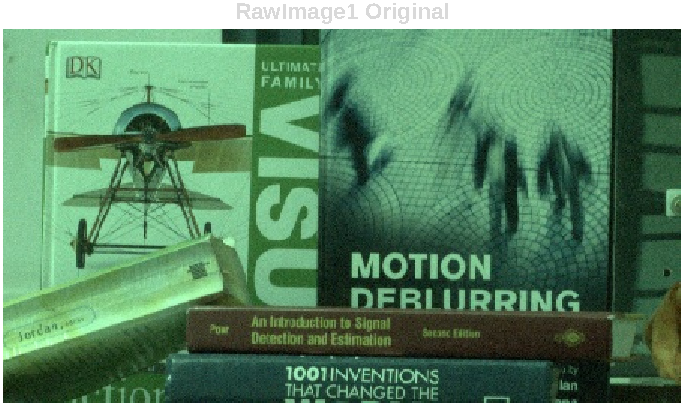
\includegraphics[width=\linewidth]{../output/RawImage1_WB_1.pdf}
							\caption{RawImage1 Original}
							\label{fig:RawImage1_WB_1}
						\end{subfigure} &
						\begin{subfigure}[h]{0.45\linewidth}
							\centering
							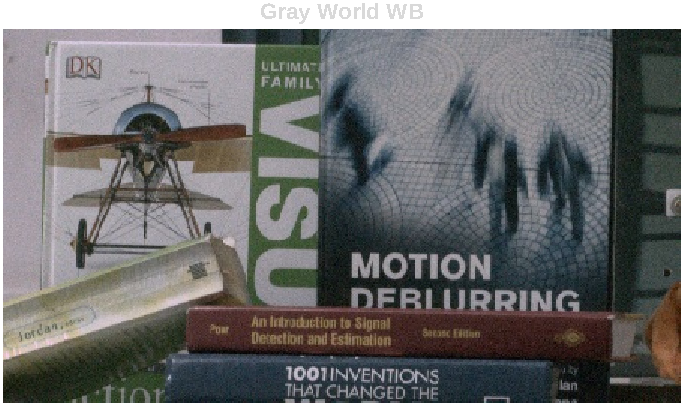
\includegraphics[width=\linewidth]{../output/RawImage1_WB_2.pdf}
							\caption{Gray World WB}
							\label{fig:RawImage1_WB_2}
						\end{subfigure}\\
						\begin{subfigure}[h]{0.45\linewidth}
							\centering
							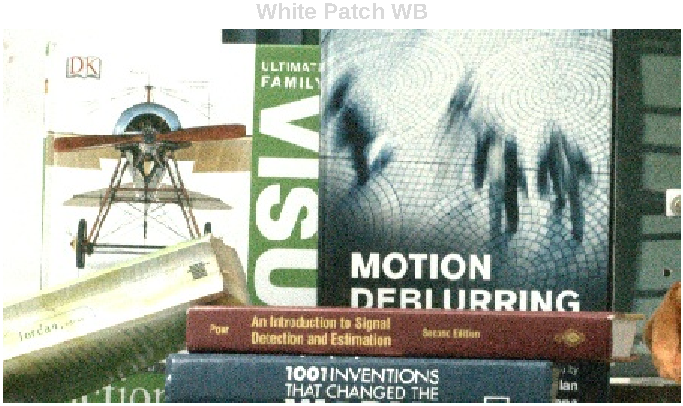
\includegraphics[width=\linewidth]{../output/RawImage1_WB_3.pdf}
							\caption{White Patch WB}
							\label{fig:RawImage1_WB_3}
						\end{subfigure} &
						\begin{subfigure}[h]{0.45\linewidth}
							\centering
							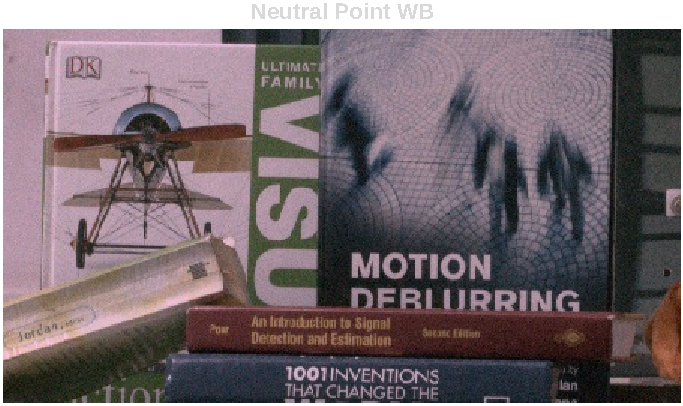
\includegraphics[width=\linewidth]{../output/RawImage1_WB_4.pdf}
							\caption{Neutral Point WB}
							\label{fig:RawImage1_WB_4}
						\end{subfigure}
					\end{tabular}
				}
				\caption{\texttt{RawImage1}-White Balance}
				\label{fig:RawImage1_WB}
			\end{figure}
			
			\begin{figure}[h]
				\centering
				\resizebox{0.8\linewidth}{!}{
					\begin{tabular}{cc}
						\begin{subfigure}[h]{0.45\linewidth}
							\centering
							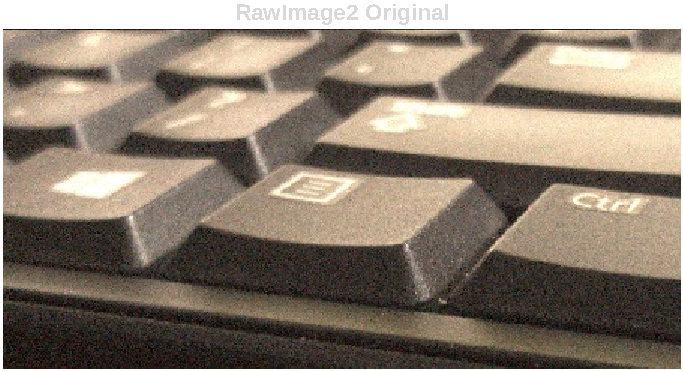
\includegraphics[width=\linewidth]{../output/RawImage2_WB_1.pdf}
							\caption{RawImage2 Original}
							\label{fig:RawImage2_WB_1}
						\end{subfigure} &
						\begin{subfigure}[h]{0.45\linewidth}
							\centering
							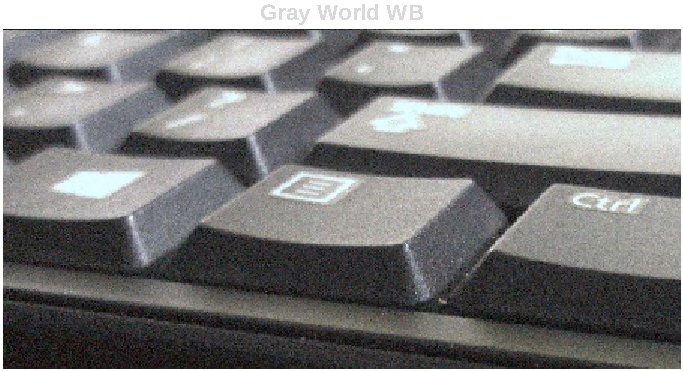
\includegraphics[width=\linewidth]{../output/RawImage2_WB_2.pdf}
							\caption{Gray World WB}
							\label{fig:RawImage2_WB_2}
						\end{subfigure}\\
						\begin{subfigure}[h]{0.45\linewidth}
							\centering
							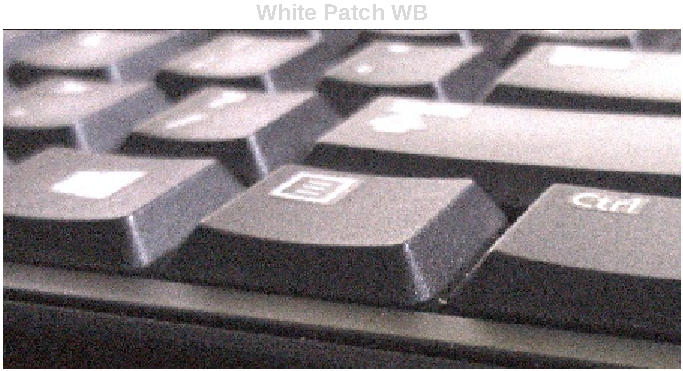
\includegraphics[width=\linewidth]{../output/RawImage2_WB_3.pdf}
							\caption{White Patch WB}
							\label{fig:RawImage2_WB_3}
						\end{subfigure} &
						\begin{subfigure}[h]{0.45\linewidth}
							\centering
							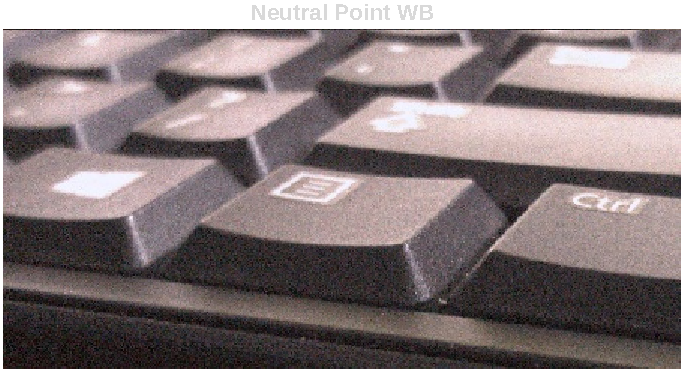
\includegraphics[width=\linewidth]{../output/RawImage2_WB_4.pdf}
							\caption{Neutral Point WB}
							\label{fig:RawImage2_WB_4}
						\end{subfigure}
					\end{tabular}
				}
				\caption{\texttt{RawImage2}-White Balance}
				\label{fig:RawImage2_WB}
			\end{figure}   
			
			\begin{figure}[h]
				\centering
				\resizebox{0.8\linewidth}{!}{
					\begin{tabular}{cc}
						\begin{subfigure}[h]{0.45\linewidth}
							\centering
							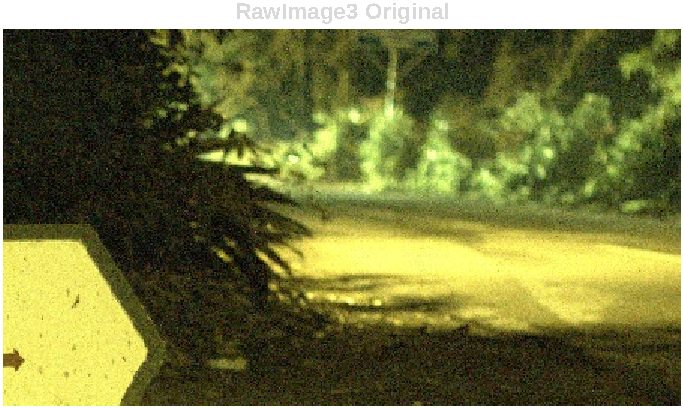
\includegraphics[width=\linewidth]{../output/RawImage3_WB_1.pdf}
							\caption{RawImage3 Original}
							\label{fig:RawImage3_WB_1}
						\end{subfigure} &
						\begin{subfigure}[h]{0.45\linewidth}
							\centering
							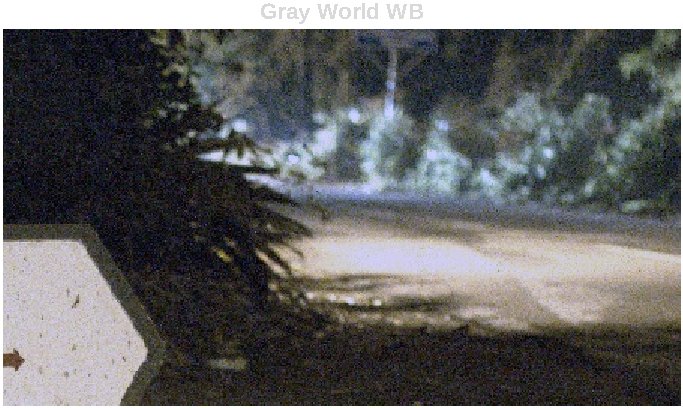
\includegraphics[width=\linewidth]{../output/RawImage3_WB_2.pdf}
							\caption{Gray World WB}
							\label{fig:RawImage3_WB_2}
						\end{subfigure}\\
						\begin{subfigure}[h]{0.45\linewidth}
							\centering
							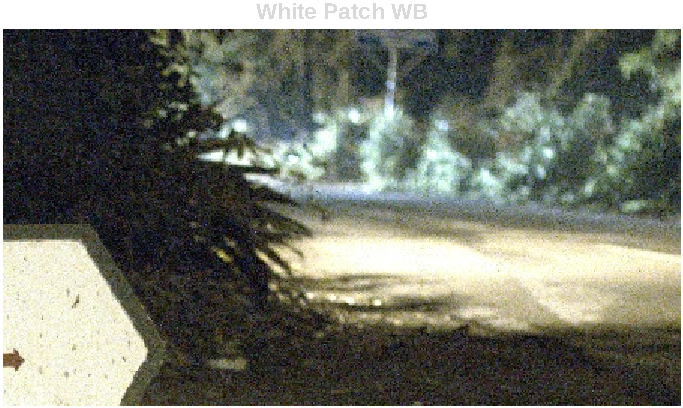
\includegraphics[width=\linewidth]{../output/RawImage3_WB_3.pdf}
							\caption{White Patch WB}
							\label{fig:RawImage3_WB_3}
						\end{subfigure} &
						\begin{subfigure}[h]{0.45\linewidth}
							\centering
							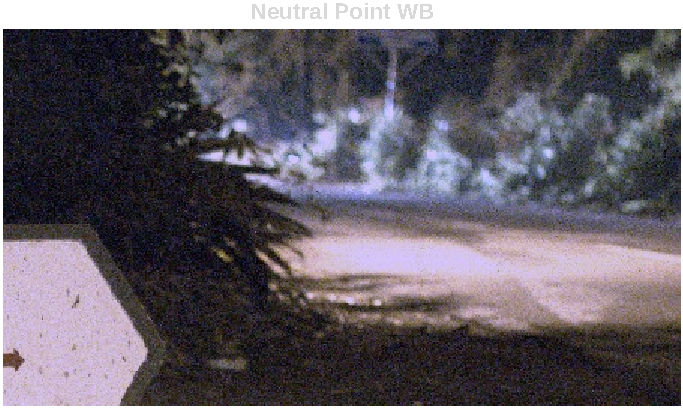
\includegraphics[width=\linewidth]{../output/RawImage3_WB_4.pdf}
							\caption{Neutral Point WB}
							\label{fig:RawImage3_WB_4}
						\end{subfigure}
					\end{tabular}
				}
				\caption{\texttt{RawImage3}-White Balance}
				\label{fig:RawImage3_WB}
			\end{figure}
			\begin{figure}[h]
				\centering
				\resizebox{\linewidth}{!}{
					\begin{tabular}{cccc}
						\begin{subfigure}[h]{0.45\linewidth}
							\centering
							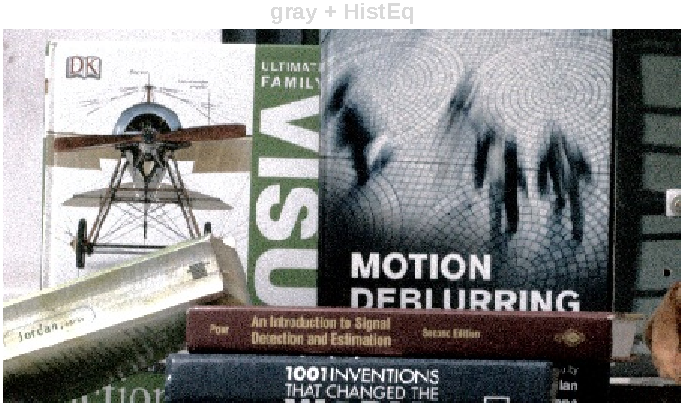
\includegraphics[width=\linewidth]{../output/RawImage1_Tone_gray_HistEq.pdf}
							\caption{gray+HistEq}
							\label{fig:RawImage1_tone_1}
						\end{subfigure} &
						\begin{subfigure}[h]{0.45\linewidth}
							\centering
							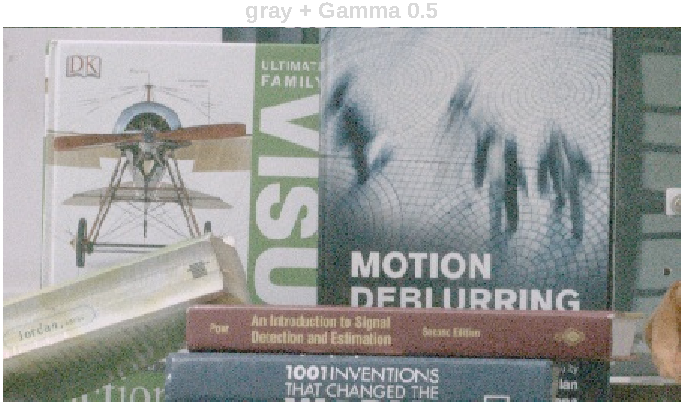
\includegraphics[width=\linewidth]{../output/RawImage1_Tone_gray_Gamma0.5.pdf}
							\caption{gray+Gamma 0.5}
							\label{fig:RawImage1_tone_2}
						\end{subfigure} &
						\begin{subfigure}[h]{0.45\linewidth}
							\centering
							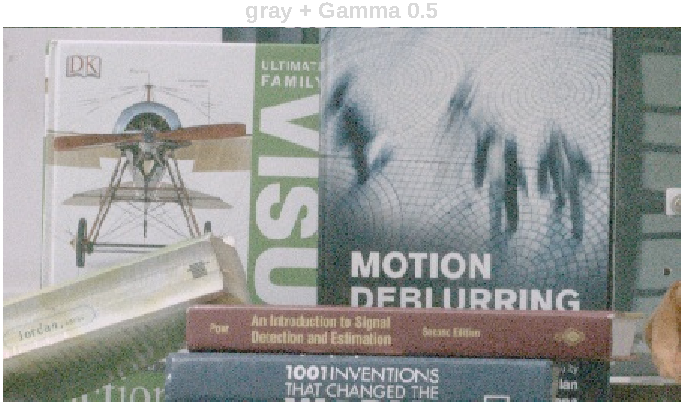
\includegraphics[width=\linewidth]{../output/RawImage1_Tone_gray_Gamma0.5.pdf}
							\caption{gray+Gamma 0.7}
							\label{fig:RawImage1_tone_3}
						\end{subfigure} &
						\begin{subfigure}[h]{0.45\linewidth}
							\centering
							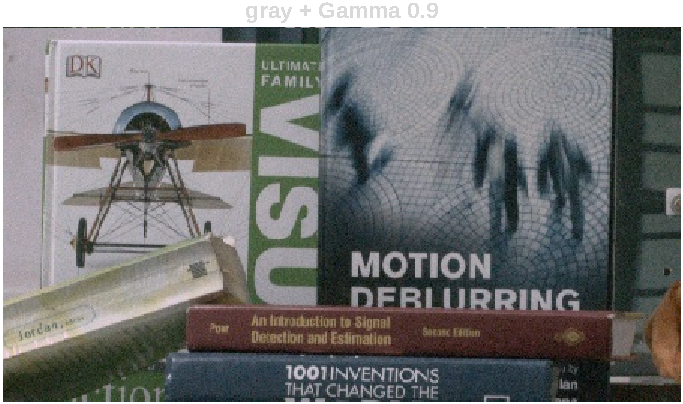
\includegraphics[width=\linewidth]{../output/RawImage1_Tone_gray_Gamma0.9.pdf}
							\caption{gray+Gamma 0.9}
							\label{fig:RawImage1_tone_4}
						\end{subfigure}\\
						\begin{subfigure}[h]{0.45\linewidth}
							\centering
							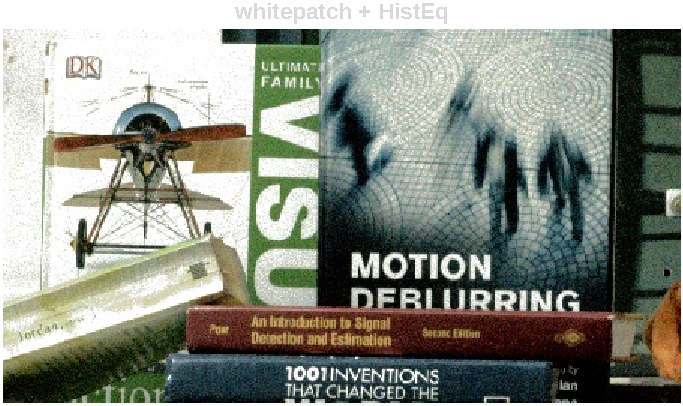
\includegraphics[width=\linewidth]{../output/RawImage1_Tone_whitepatch_HistEq.pdf}
							\caption{whitepatch+HistEq}
							\label{fig:RawImage1_tone_5}
						\end{subfigure} &
						\begin{subfigure}[h]{0.45\linewidth}
							\centering
							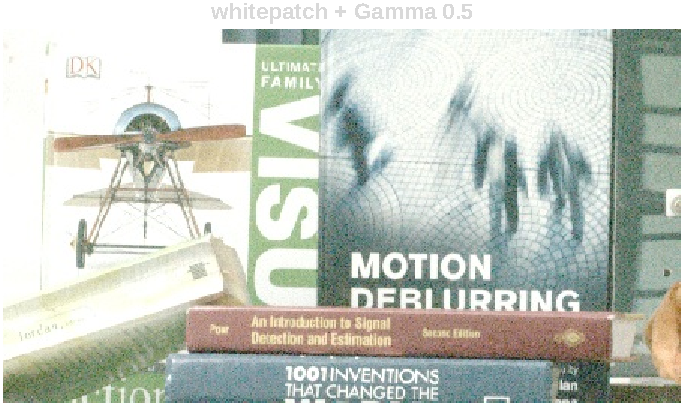
\includegraphics[width=\linewidth]{../output/RawImage1_Tone_whitepatch_Gamma0.5.pdf}
							\caption{whitepatch+Gamma 0.5}
							\label{fig:RawImage1_tone_6}
						\end{subfigure} &
						\begin{subfigure}[h]{0.45\linewidth}
							\centering
							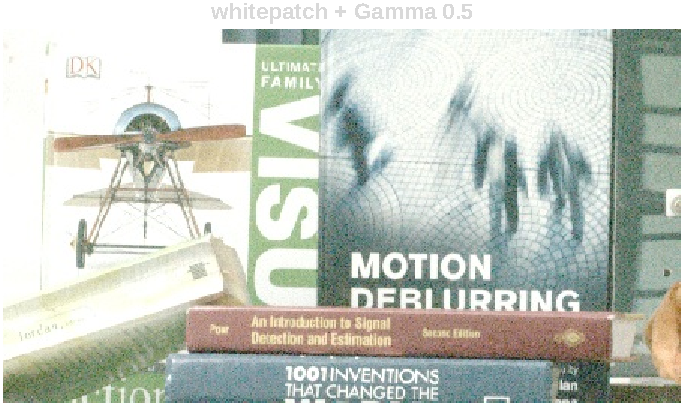
\includegraphics[width=\linewidth]{../output/RawImage1_Tone_whitepatch_Gamma0.5.pdf}
							\caption{whitepatch+Gamma 0.7}
							\label{fig:RawImage1_tone_7}
						\end{subfigure} &
						\begin{subfigure}[h]{0.45\linewidth}
							\centering
							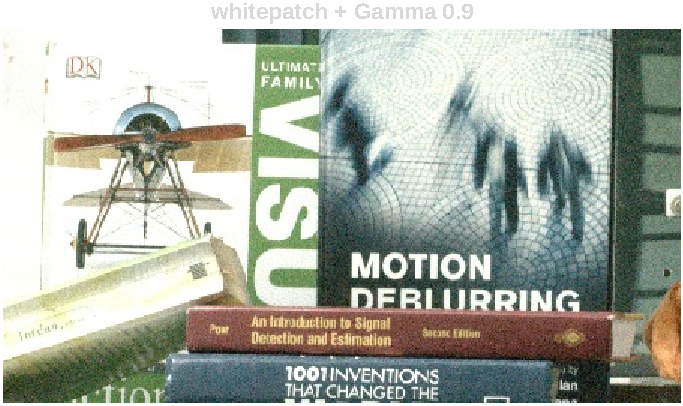
\includegraphics[width=\linewidth]{../output/RawImage1_Tone_whitepatch_Gamma0.9.pdf}
							\caption{whitepatch+Gamma 0.9}
							\label{fig:RawImage1_tone_8}
						\end{subfigure}\\
						\begin{subfigure}[h]{0.45\linewidth}
							\centering
							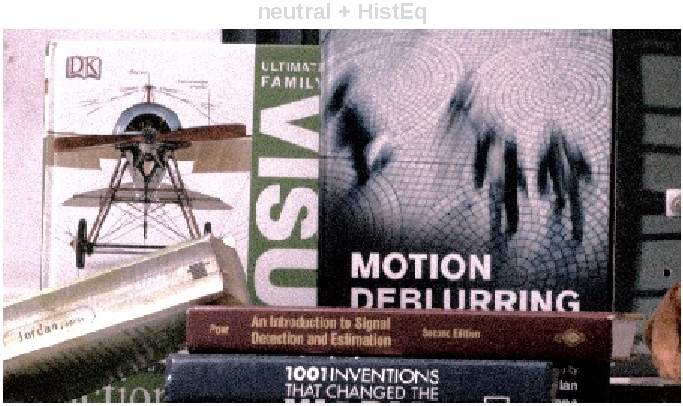
\includegraphics[width=\linewidth]{../output/RawImage1_Tone_neutral_HistEq.pdf}
							\caption{neutral+HistEq}
							\label{fig:RawImage1_tone_9}
						\end{subfigure} &
						\begin{subfigure}[h]{0.45\linewidth}
							\centering
							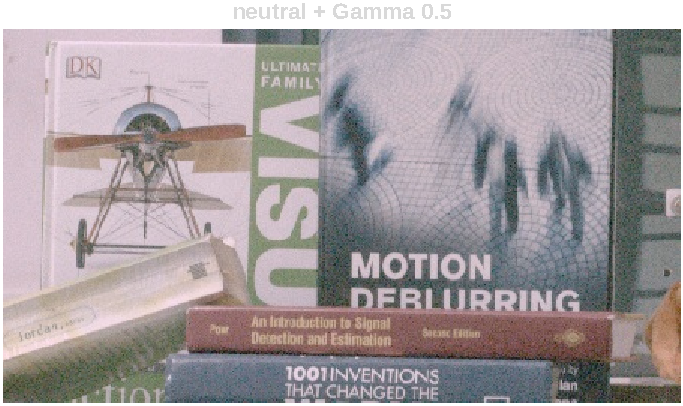
\includegraphics[width=\linewidth]{../output/RawImage1_Tone_neutral_Gamma0.5.pdf}
							\caption{neutral+Gamma 0.5}
							\label{fig:RawImage1_tone_10}
						\end{subfigure} &
						\begin{subfigure}[h]{0.45\linewidth}
							\centering
							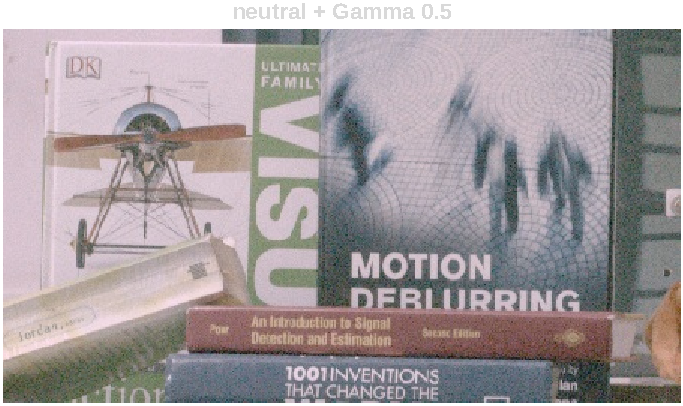
\includegraphics[width=\linewidth]{../output/RawImage1_Tone_neutral_Gamma0.5.pdf}
							\caption{neutral+Gamma 0.7}
							\label{fig:RawImage1_tone_11}
						\end{subfigure} &
						\begin{subfigure}[h]{0.45\linewidth}
							\centering
							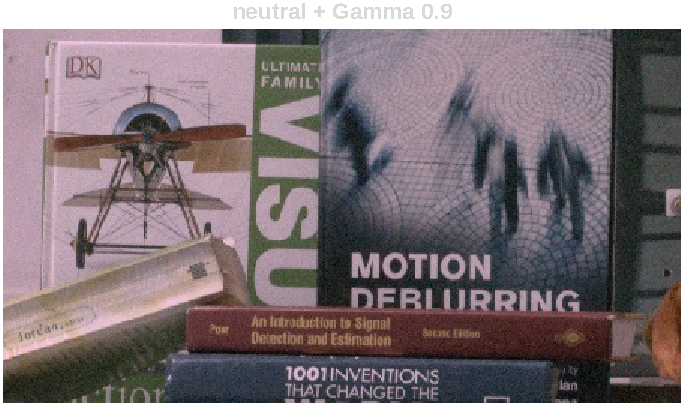
\includegraphics[width=\linewidth]{../output/RawImage1_Tone_neutral_Gamma0.9.pdf}
							\caption{neutral+Gamma 0.9}
							\label{fig:RawImage1_tone_12}
						\end{subfigure}
					\end{tabular}
				}
				\caption{\texttt{RawImage1}-tone mapping}
				\label{fig:RawImage1_tone}
			\end{figure}
			\begin{figure}[h]
				\centering
				\resizebox{\linewidth}{!}{
					\begin{tabular}{cccc}
						\begin{subfigure}[h]{0.45\linewidth}
							\centering
							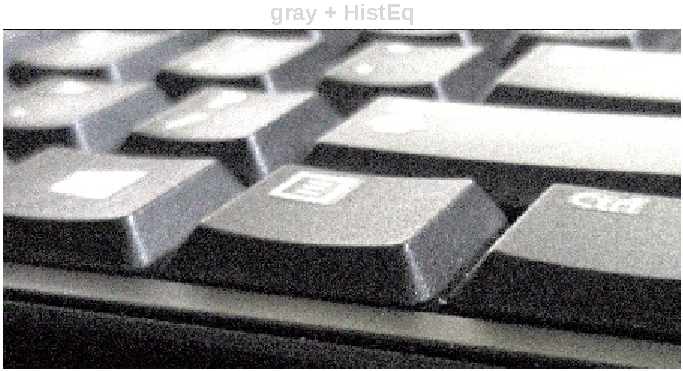
\includegraphics[width=\linewidth]{../output/RawImage2_Tone_gray_HistEq.pdf}
							\caption{gray+HistEq}
							\label{fig:RawImage2_tone_1}
						\end{subfigure} &
						\begin{subfigure}[h]{0.45\linewidth}
							\centering
							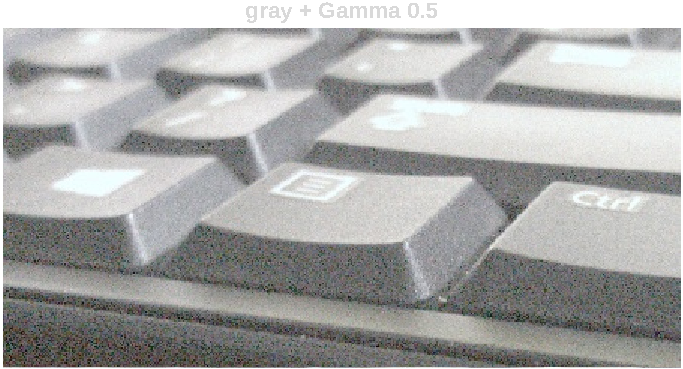
\includegraphics[width=\linewidth]{../output/RawImage2_Tone_gray_Gamma0.5.pdf}
							\caption{gray+Gamma 0.5}
							\label{fig:RawImage2_tone_2}
						\end{subfigure} &
						\begin{subfigure}[h]{0.45\linewidth}
							\centering
							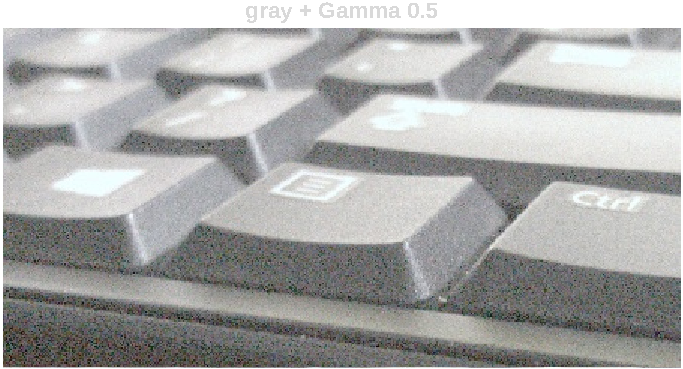
\includegraphics[width=\linewidth]{../output/RawImage2_Tone_gray_Gamma0.5.pdf}
							\caption{gray+Gamma 0.7}
							\label{fig:RawImage2_tone_3}
						\end{subfigure} &
						\begin{subfigure}[h]{0.45\linewidth}
							\centering
							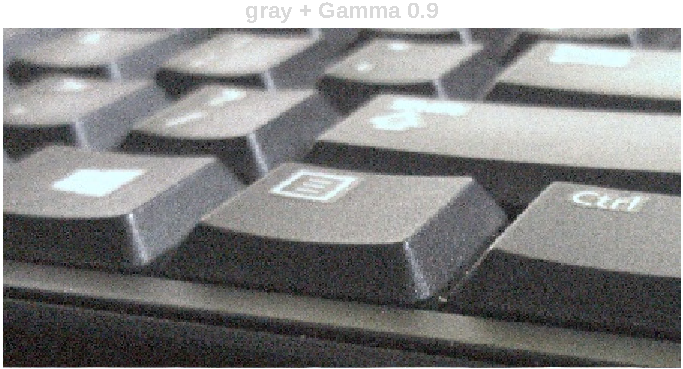
\includegraphics[width=\linewidth]{../output/RawImage2_Tone_gray_Gamma0.9.pdf}
							\caption{gray+Gamma 0.9}
							\label{fig:RawImage2_tone_4}
						\end{subfigure}\\
						\begin{subfigure}[h]{0.45\linewidth}
							\centering
							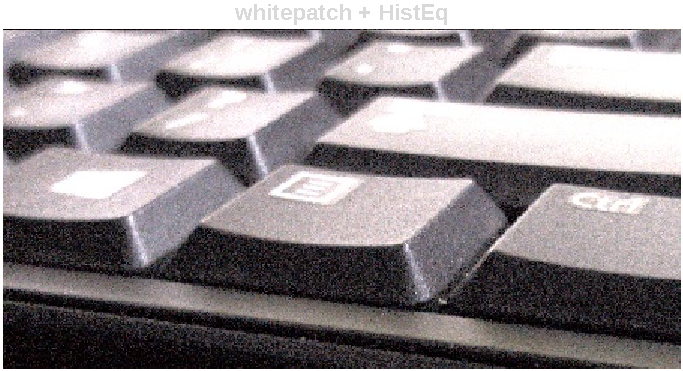
\includegraphics[width=\linewidth]{../output/RawImage2_Tone_whitepatch_HistEq.pdf}
							\caption{whitepatch+HistEq}
							\label{fig:RawImage2_tone_5}
						\end{subfigure} &
						\begin{subfigure}[h]{0.45\linewidth}
							\centering
							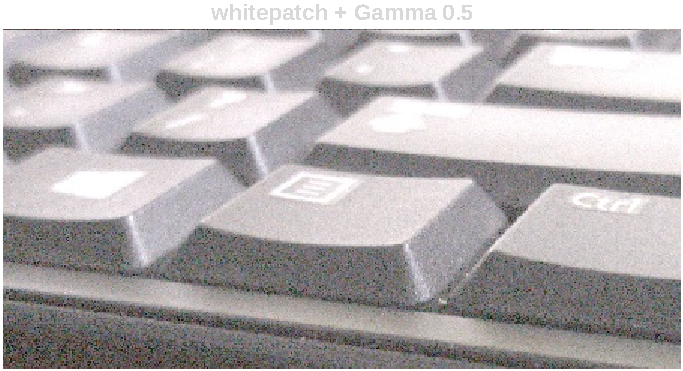
\includegraphics[width=\linewidth]{../output/RawImage2_Tone_whitepatch_Gamma0.5.pdf}
							\caption{whitepatch+Gamma 0.5}
							\label{fig:RawImage2_tone_6}
						\end{subfigure} &
						\begin{subfigure}[h]{0.45\linewidth}
							\centering
							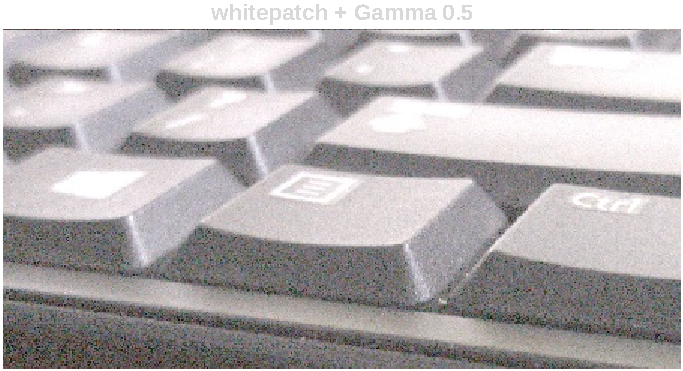
\includegraphics[width=\linewidth]{../output/RawImage2_Tone_whitepatch_Gamma0.5.pdf}
							\caption{whitepatch+Gamma 0.7}
							\label{fig:RawImage2_tone_7}
						\end{subfigure} &
						\begin{subfigure}[h]{0.45\linewidth}
							\centering
							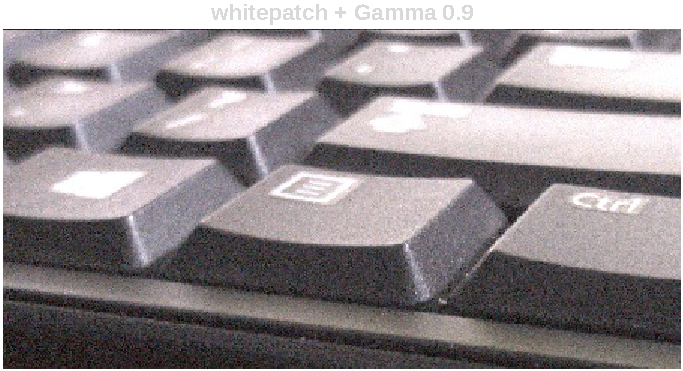
\includegraphics[width=\linewidth]{../output/RawImage2_Tone_whitepatch_Gamma0.9.pdf}
							\caption{whitepatch+Gamma 0.9}
							\label{fig:RawImage2_tone_8}
						\end{subfigure}\\
						\begin{subfigure}[h]{0.45\linewidth}
							\centering
							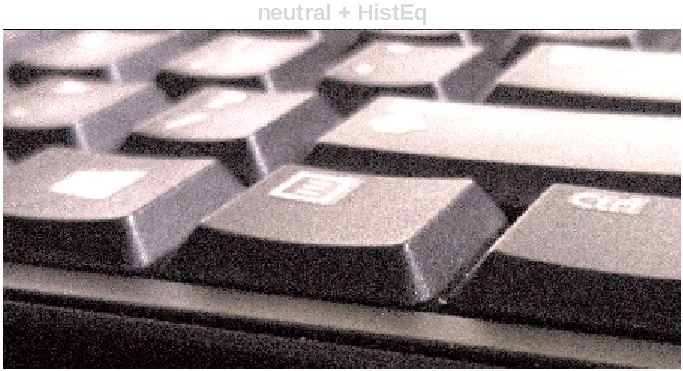
\includegraphics[width=\linewidth]{../output/RawImage2_Tone_neutral_HistEq.pdf}
							\caption{neutral+HistEq}
							\label{fig:RawImage2_tone_9}
						\end{subfigure} &
						\begin{subfigure}[h]{0.45\linewidth}
							\centering
							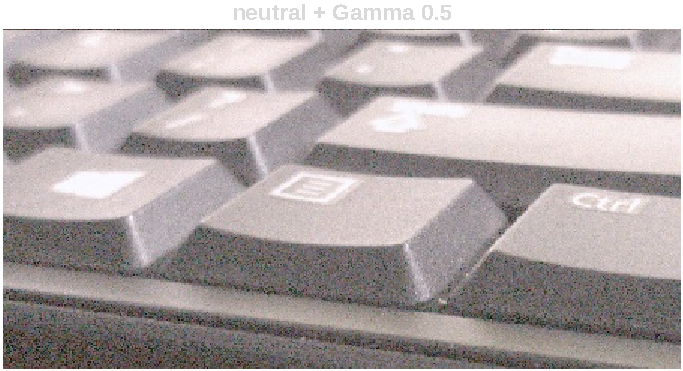
\includegraphics[width=\linewidth]{../output/RawImage2_Tone_neutral_Gamma0.5.pdf}
							\caption{neutral+Gamma 0.5}
							\label{fig:RawImage2_tone_10}
						\end{subfigure} &
						\begin{subfigure}[h]{0.45\linewidth}
							\centering
							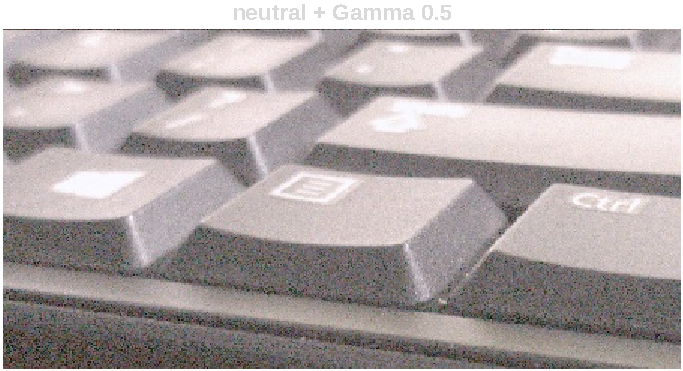
\includegraphics[width=\linewidth]{../output/RawImage2_Tone_neutral_Gamma0.5.pdf}
							\caption{neutral+Gamma 0.7}
							\label{fig:RawImage2_tone_11}
						\end{subfigure} &
						\begin{subfigure}[h]{0.45\linewidth}
							\centering
							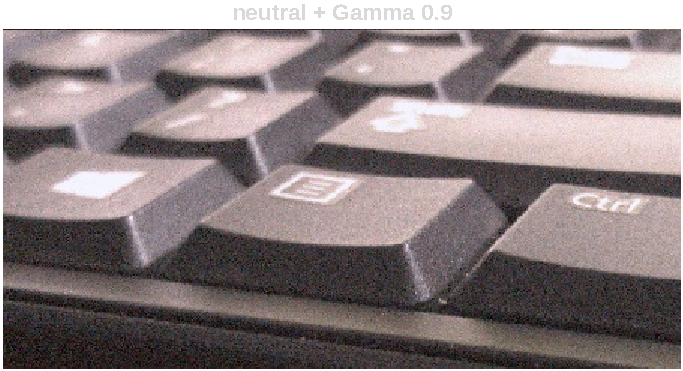
\includegraphics[width=\linewidth]{../output/RawImage2_Tone_neutral_Gamma0.9.pdf}
							\caption{neutral+Gamma 0.9}
							\label{fig:RawImage2_tone_12}
						\end{subfigure}
					\end{tabular}
				}
				\caption{\texttt{RawImage2}-tone mapping}
				\label{fig:RawImage2_tone}
			\end{figure}
			\begin{figure}[h]
				\centering
				\resizebox{\linewidth}{!}{
					\begin{tabular}{cccc}
						\begin{subfigure}[h]{0.45\linewidth}
							\centering
							\includegraphics[width=\linewidth]{../output/RawImage3_Tone_gray_HistEq.pdf}
							\caption{gray+HistEq}
							\label{fig:RawImage3_tone_1}
						\end{subfigure} &
						\begin{subfigure}[h]{0.45\linewidth}
							\centering
							\includegraphics[width=\linewidth]{../output/RawImage3_Tone_gray_Gamma0.5.pdf}
							\caption{gray+Gamma 0.5}
							\label{fig:RawImage3_tone_2}
						\end{subfigure} &
						\begin{subfigure}[h]{0.45\linewidth}
							\centering
							\includegraphics[width=\linewidth]{../output/RawImage3_Tone_gray_Gamma0.5.pdf}
							\caption{gray+Gamma 0.7}
							\label{fig:RawImage3_tone_3}
						\end{subfigure} &
						\begin{subfigure}[h]{0.45\linewidth}
							\centering
							\includegraphics[width=\linewidth]{../output/RawImage3_Tone_gray_Gamma0.9.pdf}
							\caption{gray+Gamma 0.9}
							\label{fig:RawImage3_tone_4}
						\end{subfigure}\\
						\begin{subfigure}[h]{0.45\linewidth}
							\centering
							\includegraphics[width=\linewidth]{../output/RawImage3_Tone_whitepatch_HistEq.pdf}
							\caption{whitepatch+HistEq}
							\label{fig:RawImage3_tone_5}
						\end{subfigure} &
						\begin{subfigure}[h]{0.45\linewidth}
							\centering
							\includegraphics[width=\linewidth]{../output/RawImage3_Tone_whitepatch_Gamma0.5.pdf}
							\caption{whitepatch+Gamma 0.5}
							\label{fig:RawImage3_tone_6}
						\end{subfigure} &
						\begin{subfigure}[h]{0.45\linewidth}
							\centering
							\includegraphics[width=\linewidth]{../output/RawImage3_Tone_whitepatch_Gamma0.5.pdf}
							\caption{whitepatch+Gamma 0.7}
							\label{fig:RawImage3_tone_7}
						\end{subfigure} &
						\begin{subfigure}[h]{0.45\linewidth}
							\centering
							\includegraphics[width=\linewidth]{../output/RawImage3_Tone_whitepatch_Gamma0.9.pdf}
							\caption{whitepatch+Gamma 0.9}
							\label{fig:RawImage3_tone_8}
						\end{subfigure}\\
						\begin{subfigure}[h]{0.45\linewidth}
							\centering
							\includegraphics[width=\linewidth]{../output/RawImage3_Tone_neutral_HistEq.pdf}
							\caption{neutral+HistEq}
							\label{fig:RawImage3_tone_9}
						\end{subfigure} &
						\begin{subfigure}[h]{0.45\linewidth}
							\centering
							\includegraphics[width=\linewidth]{../output/RawImage3_Tone_neutral_Gamma0.5.pdf}
							\caption{neutral+Gamma 0.5}
							\label{fig:RawImage3_tone_10}
						\end{subfigure} &
						\begin{subfigure}[h]{0.45\linewidth}
							\centering
							\includegraphics[width=\linewidth]{../output/RawImage3_Tone_neutral_Gamma0.5.pdf}
							\caption{neutral+Gamma 0.7}
							\label{fig:RawImage3_tone_11}
						\end{subfigure} &
						\begin{subfigure}[h]{0.45\linewidth}
							\centering
							\includegraphics[width=\linewidth]{../output/RawImage3_Tone_neutral_Gamma0.9.pdf}
							\caption{neutral+Gamma 0.9}
							\label{fig:RawImage3_tone_12}
						\end{subfigure}
					\end{tabular}
				}
				\caption{\texttt{RawImage3}-tone mapping}
				\label{fig:RawImage3_tone}
			\end{figure}
		\end{enumerate}
	\end{enumerate}
\end{document}